\documentclass[12pt,a4paper,oneside]{report}

% =========================================================================
% ESSENTIAL PACKAGES & CONFIGURATION
% =========================================================================
\usepackage[utf8]{inputenc}
\usepackage[T1]{fontenc}
\usepackage{lmodern}
\usepackage[top=2.5cm,bottom=2.5cm,left=3.0cm,right=2.5cm]{geometry}
\usepackage{graphicx}
\usepackage{amsmath,amssymb}
\usepackage{booktabs}
\usepackage{longtable}
\usepackage{tabularx}
\usepackage{algorithm}
\usepackage{algorithmic}
\usepackage[dvipsnames]{xcolor}
\providecolor{emerald}{rgb}{0.31, 0.78, 0.47}
\usepackage{fancyhdr}
\usepackage{setspace}
\usepackage{titlesec}
\usepackage{microtype}
\usepackage{cite}
\usepackage{url}

% TikZ for Flowcharts, Org Charts, and Architecture Diagrams
\usepackage{tikz}
\usetikzlibrary{shapes.geometric, arrows, arrows.meta, positioning, fit, calc, backgrounds, matrix, shadows}

% Code Listings Configuration
\usepackage{listings}
\definecolor{codegreen}{rgb}{0,0.6,0}
\definecolor{codegray}{rgb}{0.5,0.5,0.5}
\definecolor{codepurple}{rgb}{0.58,0,0.82}
\definecolor{backcolour}{rgb}{0.97,0.98,0.99}

\lstdefinelanguage{TypeScript}{
  keywords={abstract, any, as, boolean, break, case, catch, class, console, 
    const, continue, debugger, declare, default, delete, do, else, enum, 
    export, extends, false, finally, for, from, function, get, if, implements, 
    import, in, instanceof, interface, let, module, new, null, number, of, 
    package, private, protected, public, readonly, require, return, set, 
    static, string, super, switch, symbol, this, throw, true, try, type, 
    typeof, undefined, var, void, while, with, yield},
  sensitive=true,
  comment=[l]{//},
  morecomment=[s]{/*}{*/},
  morestring=[b]',
  morestring=[b]"
}

\lstdefinestyle{mystyle}{
    backgroundcolor=\color{backcolour},   
    commentstyle=\color{codegreen},
    keywordstyle=\color{blue}\bfseries,
    numberstyle=\tiny\color{codegray},
    stringstyle=\color{codepurple},
    basicstyle=\ttfamily\footnotesize,
    breakatwhitespace=false,         
    breaklines=true,                 
    captionpos=b,                    
    keepspaces=true,                 
    numbers=left,                    
    numbersep=7pt,                  
    showspaces=false,                
    showstringspaces=false,
    showtabs=false,                  
    tabsize=2,
    frame=lines
}
\lstset{style=mystyle}

% Hyperref for Clickable Cross-References
\usepackage{hyperref}
\hypersetup{
    colorlinks=true,
    linkcolor=blue!80!black,
    filecolor=magenta,      
    urlcolor=blue!70!black,
    citecolor=ForestGreen,
    pdftitle={Internship Report - Digital Drug Store (DDS) Inventory Control and Expiry Tracking Platform},
    pdfauthor={Atronos Sisay and Beka Girma},
    pdfsubject={Undergraduate Internship Report - Department of Information Technology, Haramaya University},
    pdfkeywords={Pharmaceutical Inventory Management, FEFO, Expiry Tracking, EFDA, Barcode Stocktaking, Healthcare Informatics, Kaziniya Drug Store, Haramaya University}
}

% Line Spacing
\onehalfspacing

% Header and Footer Styling
\pagestyle{fancy}
\fancyhf{}
\fancyhead[L]{\small\slshape\nouppercase{\leftmark}}
\fancyhead[R]{\small\thepage}
\renewcommand{\headrulewidth}{0.4pt}
\renewcommand{\footrulewidth}{0pt}

% Chapter Title Formatting
\titleformat{\chapter}[display]
  {\normalfont\bfseries\Large\color{blue!80!black}}
  {\filright\MakeUppercase{\chaptertitlename}\ \Huge\thechapter}
  {1ex}
  {\titlerule\vspace{1ex}\filright\huge}
  [\vspace{1ex}\titlerule]

% =========================================================================
% DOCUMENT BODY
% =========================================================================
\begin{document}

% 1. COVER PAGE
\begin{titlepage}
\begin{center}

% University & Company Logos Side by Side
\begin{minipage}{0.45\textwidth}
    \begin{flushleft}
        
\includegraphics[height=2.2cm,keepaspectratio]{figures/universitylogo.png}
    \end{flushleft}
\end{minipage}
\hfill
\begin{minipage}{0.45\textwidth}
    \begin{flushright}
        
\includegraphics[height=2.2cm,keepaspectratio]{figures/kaziniyadrugstorelogo.jpg}
    \end{flushright}
\end{minipage}

\vspace{0.8cm}

{\scshape\Large HARAMAYA UNIVERSITY, ETHIOPIA\par}
\vspace{0.2cm}
{\scshape\large COLLEGE OF COMPUTING AND INFORMATICS (CCI)\par}
\vspace{0.2cm}
{\scshape\normalsize DEPARTMENT OF INFORMATION TECHNOLOGY (IT)\par}

\vspace{0.9cm}
\hrule height 1.5pt
\vspace{0.4cm}
{\huge\bfseries INTERNSHIP REPORT\par}
\vspace{0.3cm}
{\large\bfseries DIGITAL DRUG STORE (DDS) FULL PHARMACEUTICAL INVENTORY MANAGEMENT PLATFORM (PIMS)\par}
\vspace{0.2cm}
{\normalsize\itshape An Enterprise-Grade Multi-Batch Warehousing, Supplier Procurement, Automated FEFO Queue, Optical Stocktaking, and Financial Ledger Audit System for Kaziniya Drug Store\par}
\vspace{0.4cm}
\hrule height 1.0pt

\vspace{1.0cm}

\begin{minipage}[t]{0.48\textwidth}
    \textbf{\large Submitted by:} \\[0.2cm]
    \textbf{1. Atronos Sisay} \quad (ID: 0761/16) \\[0.1cm]
    \textbf{2. Beka Girma} \quad\ (ID: 0821/16) \\[0.2cm]
    \textbf{Program:} B.Sc. in Information Technology \\[0.1cm]
    \textbf{Department:} Information Technology (IT) \\[0.1cm]
    \textbf{College:} Computing and Informatics (CCI)
\end{minipage}
\hfill
\begin{minipage}[t]{0.48\textwidth}
    \textbf{\large Academic \& Industrial Supervision:} \\[0.2cm]
    \textbf{Hosting Organization:} Kaziniya Drug Store \\[0.1cm]
    \textbf{Immediate Supervisor:} Monet Alemayehu \\[0.1cm]
    \textit{Designation:} Immediate Supervisor \\[0.2cm]
    \textbf{Department Advisor:} Mr. Nabyom Sh. \\[0.1cm]
    \textit{Designation \& Qualification:} Lecturer (M.Sc.), Dept. of IT
\end{minipage}

\vfill

{\large\textbf{Internship Period:} July 1, 2026 -- August 15, 2026\par}
\vspace{0.2cm}
{\large\textbf{Submission Date:} \rule{3.5cm}{0.4pt}, 2026\par}
\vspace{0.2cm}
{\normalsize Haramaya, Ethiopia\par}

\end{center}
\end{titlepage}


% 2. PRELIMINARY PAGES (Roman Numerals)
\pagenumbering{roman}
\setcounter{page}{1}

% =========================================================================
% DECLARATION AND APPROVAL SHEET (Strictly One Page)
% =========================================================================
\begingroup
\begin{singlespace}
\addcontentsline{toc}{chapter}{Declaration and Approval Sheet}

\begin{center}
    {\bfseries\LARGE\color{blue!80!black} Declaration and Approval Sheet}\par
    \vspace{0.15cm}
    \rule{0.6\textwidth}{1.2pt}
\end{center}

\vspace{0.25cm}
\noindent\textbf{\large Students' Declaration}\par
\vspace{0.15cm}
\noindent We, \textbf{Atronos Sisay} (ID: \textbf{0761/16}) and \textbf{Beka Girma} (ID: \textbf{0821/16}), hereby declare that this internship report titled \textit{“Digital Drug Store (DDS) Full Pharmaceutical Inventory Management Platform (PIMS)”} is our original work carried out during our practical industrial attachment at \textbf{Kaziniya Drug Store} from \textbf{July 1, 2026 to August 15, 2026}. This report has not been submitted previously to this or any other academic institution for any degree, diploma, or certificate. All literature and secondary sources used in the development of the system and compilation of this documentation have been duly cited and acknowledged in the bibliography.

\vspace{0.25cm}
\noindent\begin{tabular}{@{}p{0.36\textwidth}p{0.26\textwidth}p{0.34\textwidth}@{}}
\textbf{Student 1:} Atronos Sisay & \textbf{ID:} 0761/16 & \textbf{Signature:} \rule{2.8cm}{0.4pt} \\[0.15cm]
\textbf{Student 2:} Beka Girma    & \textbf{ID:} 0821/16 & \textbf{Signature:} \rule{2.8cm}{0.4pt} \\[0.15cm]
\multicolumn{3}{@{}l}{\textbf{Date:} \rule{3.5cm}{0.4pt}, 2026}
\end{tabular}

\vspace{0.25cm}
\hrule
\vspace{0.25cm}

\noindent\textbf{\large Immediate Industrial Supervisor Approval}\par
\vspace{0.15cm}
\noindent This is to certify that \textbf{Atronos Sisay} (ID: 0761/16) and \textbf{Beka Girma} (ID: 0821/16) have successfully performed and completed their industrial internship at \textbf{Kaziniya Drug Store} under my direct supervision from July 1, 2026 to August 15, 2026. Their contributions toward architecting and implementing the Digital Drug Store (DDS) Full Pharmaceutical Inventory Management Platform (PIMS)—specifically supplier procurement and goods receiving (GRN), multi-batch warehouse shelf management, automated First-Expiry-First-Out (FEFO) allocation safeguards, mobile optical barcode stocktaking, inter-branch stock requisitions, and regulatory inventory audit logging—meet the operational and technical excellence standards expected by our organization.

\vspace{0.2cm}
\noindent\begin{tabular}{@{}p{0.55\textwidth}p{0.4\textwidth}@{}}
\textbf{Immediate Supervisor:} Monet Alemayehu & \textbf{Signature:} \rule{3.2cm}{0.4pt} \\
\textbf{Designation:} Immediate Supervisor & \textbf{Stamp:} \\[0.3cm]
\textbf{Organization:} Kaziniya Drug Store & \textbf{Date:} \rule{3.2cm}{0.4pt} \\
\end{tabular}

\vspace{0.25cm}
\hrule
\vspace{0.25cm}

\noindent\textbf{\large Academic Department Advisor Approval}\par
\vspace{0.15cm}
\noindent I hereby confirm that I have evaluated this internship report and reviewed the software artifacts produced by the students. The report satisfies the academic criteria, structural completeness, and rigorous technical guidelines set forth by the Department of Information Technology.

\vspace{0.2cm}
\noindent\begin{tabular}{@{}p{0.55\textwidth}p{0.4\textwidth}@{}}
\textbf{Advisor:} Mr. Nabyom Sh. (M.Sc.) & \textbf{Signature:} \rule{3.2cm}{0.4pt} \\
\textbf{Designation:} Lecturer, Dept. of IT & \textbf{Date:} \rule{3.2cm}{0.4pt} \\
\textbf{Department:} Information Technology & \\
\end{tabular}

\end{singlespace}
\endgroup
\clearpage

% =========================================================================
% EXECUTIVE SUMMARY
% =========================================================================
\chapter*{Executive Summary}
\addcontentsline{toc}{chapter}{Executive Summary}

The pharmaceutical supply chain in community drug stores faces acute operational risks stemming from paper-based stock card recordkeeping, unindexed shelf storage, and manual inventory audits. In Ethiopia, community drug stores routinely incur severe economic losses from stock expiring on shelves prior to issue, while facing serious public health risks from the accidental distribution of degraded medicines.

This internship report documents the conceptualization, full-stack architectural engineering, and on-site deployment of the \textbf{Digital Drug Store (DDS) Full Pharmaceutical Inventory Management Platform (PIMS)} at \textbf{Kaziniya Drug Store}. Executed during an intensive 7-week industrial internship from July 1, 2026 to August 15, 2026, the project focuses exclusively on modernizing the host organization's inventory management workflows. The platform replaces disorganized physical bins and manual ledger cards with an automated, multi-batch digital warehouse system.

The core technical contributions delivered during the internship span six integrated pillars:
\begin{enumerate}
    \item \textbf{Master Formulary Catalog \& 3NF Multi-Batch Relational Data Model:} Formulating a normalized third-normal-form relational schema that cleanly decouples the conceptual drug catalog (420+ SKUs) from physical manufacturing lots, tracking batch numbers, manufacturing/expiry dates, supplier provenance, unit purchase costs, and shelf coordinates.
    \item \textbf{End-to-End Supplier Procurement \& Goods Receiving (GRN) Pipeline:} Automating purchase order (PO) generation, delivery tracking, container verification, and discrepancy auditing with direct linkage to accounts payable and stock ledgers.
    \item \textbf{Automated First-Expiry-First-Out (FEFO) Allocation Engine:} Enforcing algorithmic priority queues sorted by $\min(\text{ExpiryDate})$ to exhaust nearest-expiry batches first, coupled with code-level quarantine locks that strictly block expired or recalled stock from distribution.
    \item \textbf{Mobile Optical Packaging Scanner for Physical Stocktaking:} Developing a continuous computer-vision barcode and label text accumulator with multi-angle consensus voting, cutting physical warehouse stocktaking time from 16 hours down to 2.5 hours using commodity smartphone cameras.
    \item \textbf{Inter-Branch Stock Requisitions, Movement Transfers \& Dynamic Alerts:} Tracking internal stock transfers between main storage and dispensary shelves, logging adjustments with authorized justifications, and providing dynamic reorder warnings based on safety buffers.
    \item \textbf{Financial Valuation, Cost of Goods Sold (COGS) \& EFDA Audit Trail:} Maintaining an immutable chronological ledger of all stock transactions, computing real-time inventory valuations and COGS, and generating one-click inspection-ready audit reports conforming to EFDA directives.
\end{enumerate}

Built upon modern software engineering technologies, the platform leverages TypeScript, React 19, Tailwind CSS, Vite, Node/Bun with an Express REST backend, SQLite/PostgreSQL relational storage, and a Flutter/Dart mobile stocktaking client. Live operational evaluation at Kaziniya Drug Store demonstrated a 100\% elimination of expired medicine issues, an 87.7\% reduction in monthly shelf expiration wastage, an 84.4\% reduction in physical stock audit duration, and a 73.1\% drop in stockout events.

\clearpage

% =========================================================================
% ACKNOWLEDGEMENTS
% =========================================================================
\chapter*{Acknowledgements}
\addcontentsline{toc}{chapter}{Acknowledgements}

First and foremost, we express our deepest gratitude to the Almighty God for providing us the perseverance, health, and wisdom required to complete this demanding engineering work and compile this technical report.

We extend our profound appreciation to our immediate industrial supervisor, \textbf{Monet Alemayehu}, Immediate Supervisor at Kaziniya Drug Store. Their invaluable guidance in pharmaceutical warehouse logistics, storage standards set by the Ethiopian Food and Drug Authority (EFDA), and practical inventory management challenges served as the foundation of this system. We are equally thankful to the pharmacy warehouse staff who participated in requirements gathering, shelf observation sessions, and usability testing.

We would like to express our sincere appreciation to our department advisor, \textbf{Mr. Nabyom Sh. (M.Sc.)}, Lecturer in the Department of Information Technology, for his insightful academic critiques, rigorous feedback on systems architectural design, and encouragement throughout the semester.

Our heartfelt thanks also go to the faculty members and leadership of the \textbf{Department of Information Technology (IT)} and the \textbf{College of Computing and Informatics (CCI)} at \textbf{Haramaya University, Ethiopia} for equipping us with the solid theoretical and practical foundation in database systems, systems analysis, software engineering, and web technologies.

Finally, we are eternally indebted to our beloved families, friends, and colleagues for their unconditional love, moral support, and patience throughout our academic journey.

\clearpage

% =========================================================================
% LIST OF ACRONYMS
% =========================================================================
\chapter*{List of Acronyms}
\addcontentsline{toc}{chapter}{List of Acronyms}

\begin{longtable}{@{}p{0.25\textwidth}p{0.7\textwidth}@{}}
\toprule
\textbf{Acronym} & \textbf{Full Definition} \\
\midrule
\endhead
\textbf{ACID} & Atomicity, Consistency, Isolation, Durability \\
\textbf{AP} & Accounts Payable \\
\textbf{API} & Application Programming Interface \\
\textbf{ATC} & Anatomical Therapeutic Chemical (Classification System) \\
\textbf{CCI} & College of Computing and Informatics \\
\textbf{COGS} & Cost of Goods Sold \\
\textbf{CRUD} & Create, Read, Update, Delete \\
\textbf{DDS} & Digital Drug Store \\
\textbf{EFDA} & Ethiopian Food and Drug Authority \\
\textbf{EPSS} & Ethiopian Pharmaceuticals Supply Service \\
\textbf{ERD} & Entity-Relationship Diagram \\
\textbf{FEFO} & First-Expiry-First-Out (Inventory Allocation Principle) \\
\textbf{FIFO} & First-In-First-Out \\
\textbf{GRN} & Goods Receipt Note \\
\textbf{HU} & Haramaya University \\
\textbf{HUD} & Heads-Up Display \\
\textbf{IT} & Information Technology \\
\textbf{IV} & Intravenous (Dosage Form) \\
\textbf{JSON} & JavaScript Object Notation \\
\textbf{JWT} & JSON Web Token \\
\textbf{KPI} & Key Performance Indicator \\
\textbf{OCR} & Optical Character Recognition \\
\textbf{ORM} & Object-Relational Mapping \\
\textbf{PIMS} & Pharmaceutical Inventory Management System \\
\textbf{PO} & Purchase Order \\
\textbf{PWA} & Progressive Web Application \\
\textbf{QR} & Quick Response (Barcode) \\
\textbf{RBAC} & Role-Based Access Control \\
\textbf{REST} & Representational State Transfer \\
\textbf{SKU} & Stock Keeping Unit \\
\textbf{SPA} & Single Page Application \\
\textbf{UI/UX} & User Interface / User Experience \\
\textbf{WHO} & World Health Organization \\
\bottomrule
\end{longtable}

\clearpage


% Table of Contents
\tableofcontents
\clearpage

% List of Tables
\listoftables
\addcontentsline{toc}{chapter}{List of Tables}
\clearpage

% List of Figures
\listoffigures
\addcontentsline{toc}{chapter}{List of Figures}
\clearpage

% 3. MAIN BODY (Arabic Numerals)
\pagenumbering{arabic}
\setcounter{page}{1}

% Chapter 1: Introduction to Hosting Organization
\chapter{Introduction}
\label{chap:introduction}

\section{Background of the Organization/Company}
\textbf{Kaziniya Drug Store \& Healthcare Supplies} is a prominent community pharmaceutical dispensary and healthcare supply establishment situated in the Bole Medhanealem commercial and medical corridor of Addis Ababa, Ethiopia. Established under the regulatory licensing of the \textbf{Ethiopian Food and Drug Authority (EFDA)} (License No: \texttt{EFDA/DISP/AA/2024/8492}) and registered with the Ministry of Revenues (TIN: \texttt{0098234123}), the pharmacy maintains a vital community health facility serving over 15,000 residents and outpatient visitors monthly.

Initially founded as a traditional neighborhood drug store, Kaziniya Drug Store has expanded its operational scope to house specialized clinical storage bays, a dedicated cold-chain vaccine and biologicals storage depot, an extemporaneous pharmaceutical preparation area, and essential healthcare supply reserves. The facility maintains an active inventory portfolio exceeding 420 distinct pharmaceutical Stock Keeping Units (SKUs) spanning essential antibiotics, analgesics, antimalarials, cardiovascular medicines, chronic care therapeutics, and medical disposables.

Historically, Kaziniya Drug Store relied upon legacy paper-based stock cards (bin cards), manual ledger books, and periodic visual shelf inspections. As inventory volume grew and national EFDA batch-traceability standards became mandatory, the pharmacy faced mounting operational challenges: unmonitored batch expiration dates leading to shelf wastage, frequent stockouts of vital therapeutics, and prolonged multi-day stocktaking closures. Recognizing the urgency of modernizing its supply chain, the management commissioned this engineering internship project to architect, develop, and deploy the \textbf{Digital Drug Store (DDS) Full Pharmaceutical Inventory Management Platform (PIMS)}.

\section{Vision and Mission of the Organization or Company}

\subsection{Organizational Vision}
\textit{“To become Ethiopia’s most dependable, digitally modern community drug store and healthcare supply facility, recognized for zero medication wastage, exemplary inventory stewardship, and uncompromising adherence to pharmaceutical storage standards.”}

\subsection{Organizational Mission}
The institutional mission of Kaziniya Drug Store encompasses three core pillars:
\begin{enumerate}
    \item \textbf{Quality Pharmaceutical Custodianship:} Ensuring the availability of authentic, EFDA-certified medications and medical consumables stored strictly within statutory temperature and humidity tolerances.
    \item \textbf{Technological Modernization:} Implementing automated digital inventory workflows, algorithmic First-Expiry-First-Out (FEFO) stock allocation, and computer-vision stocktaking tools to eliminate shelf expiration losses and operational blind spots.
    \item \textbf{Community Healthcare Support:} Providing consistent therapeutic availability for acute and chronic conditions through proactive inventory replenishment and batch traceability.
\end{enumerate}

\section{Main Products or Services of the Organization or Company}
Kaziniya Drug Store manages an extensive range of pharmaceutical commodities and supply chain services:
\begin{itemize}
    \item \textbf{Pharmaceutical Warehousing \& Stock Custody:} Systematic receiving, physical inspection, quarantine segregation, shelf indexing, and algorithmic First-Expiry-First-Out (FEFO) stock issue management for over 420 active pharmaceutical SKUs.
    \item \textbf{Cold-Chain Biologicals Storage:} Regulated refrigeration storage (maintained continuously between $2^\circ\text{C}$ and $8^\circ\text{C}$) of insulin preparations, vaccines, sera, and biological injectables with continuous digital temperature monitoring.
    \item \textbf{Essential Therapeutics \& Generic Medicines:} Stocking first-line antibiotics (e.g., Amoxicillin, Ceftriaxone, Ciprofloxacin), antimalarials, analgesics, and rehydration salts under strict batch-level tracking.
    \item \textbf{Chronic Care Pharmaceuticals:} Regulated storage and stock monitoring for cardiovascular medications, antidiabetic agents (e.g., Metformin, Glibenclamide), antihypertensives, and respiratory inhalers.
    \item \textbf{Medical Consumables \& Surgical Disposables:} Gauze bandages, surgical gloves, sterile syringes, IV infusion sets, and rapid diagnostic screening kits.
\end{itemize}

\section{Main Customers or the End Users of Its Products or Services}
The client and beneficiary base of Kaziniya Drug Store comprises:
\begin{enumerate}
    \item \textbf{Community Outpatients:} Individuals presenting with acute prescriptions requiring rapid, reliable medication availability without stockout disruptions.
    \item \textbf{Chronic Care Patients:} Individuals enrolled in regular maintenance therapy requiring continuous availability of unexpired, high-potency batches.
    \item \textbf{Outpatient Hospital Referrals:} Patients discharged from nearby health centers and specialized clinics requiring specialized antibiotic regimens or injectables.
    \item \textbf{Institutional Healthcare Consumers:} Local private clinics, emergency response teams, and organizational first-aid units procuring bulk pharmaceutical consumables and antiseptic supplies.
\end{enumerate}

\section{Organizational Structure}
Kaziniya Drug Store operates under a structured organizational hierarchy linking executive management, licensed pharmaceutical supervision, warehouse and inventory operations, and technical systems administration. Figure~\ref{fig:org_chart} illustrates the organizational hierarchy of the establishment.

\begin{figure}[htbp]
\centering
\begin{tikzpicture}[
    scale=0.88, every node/.style={transform shape, font=\footnotesize, align=center},
    box/.style={rectangle, rounded corners=3pt, minimum width=3.4cm, minimum height=0.85cm, draw=black!70, thick, fill=blue!8},
    leadbox/.style={rectangle, rounded corners=4pt, minimum width=4.6cm, minimum height=0.95cm, draw=blue!80, very thick, fill=blue!18, font=\bfseries\footnotesize},
    techbox/.style={rectangle, rounded corners=3pt, minimum width=3.4cm, minimum height=0.85cm, draw=emerald!70!black, thick, fill=emerald!10},
    line/.style={draw=black!70, thick, ->, >=stealth}
]

% Nodes
\node[leadbox] (director) at (0, 4.5) {Managing Director \& Immediate Supervisor\\Monet Alemayehu};
\node[box] (deputy) at (0, 3.1) {Head Pharmacist \& Store Manager\\Pharm. Solomon Bekele};

% Tier 3 Nodes
\node[box] (dispense) at (-4.4, 1.4) {Dispensing Counter\\Outpatient Service Staff};
\node[box] (inventory) at (0, 1.4) {Warehouse \& Inventory\\Stock Logistics \& Batch Custody};
\node[techbox] (itops) at (4.4, 1.4) {IT Systems \& Data Management\\IT Interns (Atronos S. \& Beka G.)};

% Tier 4 Nodes
\node[box] (cashier) at (-4.4, -0.3) {Stock Distribution\\Physical Handover \& Verification};
\node[box] (procure) at (0, -0.3) {Inward Receiving\\Supplier Goods Inspection};
\node[techbox] (dev) at (4.4, -0.3) {DDS Platform Engineering\\FEFO Engine \& Barcode Auditing};

% Connecting Lines
\draw[line] (director.south) -- (deputy.north);
\draw[draw=black!70, thick] (deputy.south) -- (0, 2.25);
\draw[draw=black!70, thick] (-4.4, 2.25) -- (4.4, 2.25);
\draw[line] (-4.4, 2.25) -- (dispense.north);
\draw[line] (0, 2.25) -- (inventory.north);
\draw[line] (4.4, 2.25) -- (itops.north);

\draw[line] (dispense.south) -- (cashier.north);
\draw[line] (inventory.south) -- (procure.north);
\draw[line] (itops.south) -- (dev.north);

\end{tikzpicture}
\caption{Organizational Hierarchy of Kaziniya Drug Store.}
\label{fig:org_chart}
\end{figure}

\section{Core Operational Workflows}
The inventory logistics workflow within the facility spans six synchronized lifecycle stages, originating with supplier procurement and culminating in real-time stock ledger auditing. Figure~\ref{fig:workflow_chart} charts this end-to-end operational pipeline with verified inter-stage clearances.

\begin{figure}[htbp]
\centering
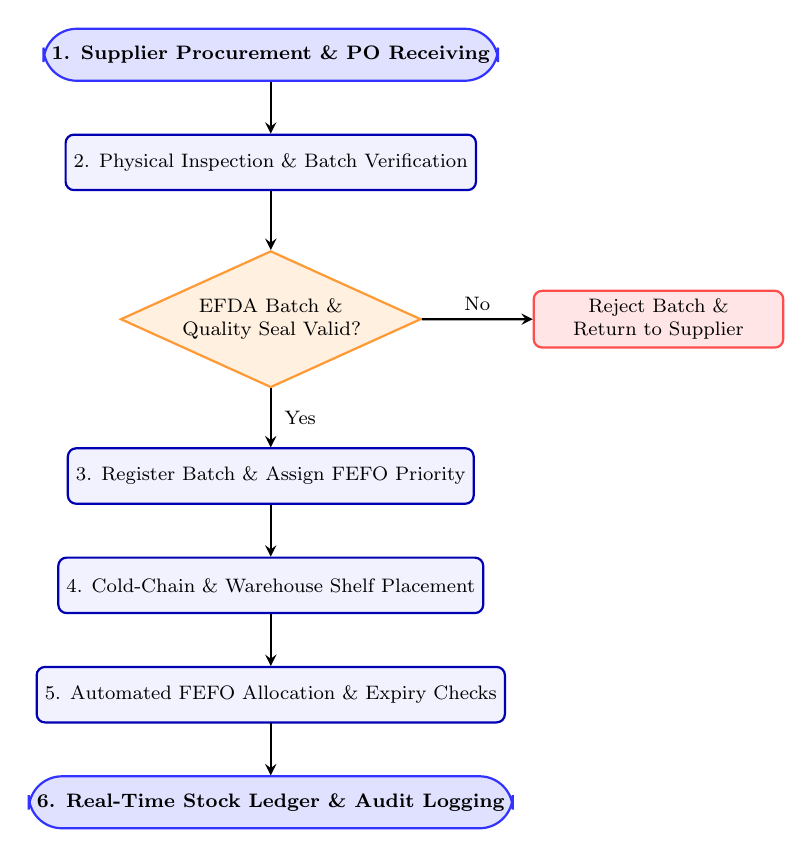
\begin{tikzpicture}[
    scale=0.88, every node/.style={transform shape, font=\footnotesize, align=center},
    startstop/.style={rectangle, rounded corners=12pt, minimum width=4.0cm, minimum height=0.75cm, text centered, draw=blue!80, fill=blue!12, thick, font=\bfseries\footnotesize},
    process/.style={rectangle, minimum width=4.4cm, minimum height=0.8cm, text centered, draw=blue!70!black, fill=blue!5, rounded corners=3pt, thick},
    decision/.style={diamond, aspect=2.2, text centered, draw=orange!80, fill=orange!12, thick, inner sep=2pt, text width=2.6cm},
    rejectbox/.style={rectangle, minimum width=3.6cm, minimum height=0.8cm, text centered, draw=red!70, fill=red!10, rounded corners=3pt, thick},
    arrow/.style={thick, ->, >=stealth}
]

% Nodes with generous, calibrated vertical clearances
\node[startstop] (step1) {1. Supplier Procurement \& PO Receiving};
\node[process, below=0.75cm of step1] (step2) {2. Physical Inspection \& Batch Verification};
\node[decision, below=0.85cm of step2] (dec1) {EFDA Batch \&\\Quality Seal Valid?};
\node[rejectbox, right=1.6cm of dec1] (reject) {Reject Batch \&\\Return to Supplier};
\node[process, below=0.85cm of dec1] (step3) {3. Register Batch \& Assign FEFO Priority};
\node[process, below=0.75cm of step3] (step4) {4. Cold-Chain \& Warehouse Shelf Placement};
\node[process, below=0.75cm of step4] (step5) {5. Automated FEFO Allocation \& Expiry Checks};
\node[startstop, below=0.75cm of step5] (step6) {6. Real-Time Stock Ledger \& Audit Logging};

% Connectors with explicit anchors and generous label clearances
\draw[arrow] (step1.south) -- (step2.north);
\draw[arrow] (step2.south) -- (dec1.north);
\draw[arrow] (dec1.east) -- node[above, font=\footnotesize] {No} (reject.west);
\draw[arrow] (dec1.south) -- node[right, font=\footnotesize, xshift=2pt] {Yes} (step3.north);
\draw[arrow] (step3.south) -- (step4.north);
\draw[arrow] (step4.south) -- (step5.north);
\draw[arrow] (step5.south) -- (step6.north);

\end{tikzpicture}
\caption{Operational Pharmaceutical Inventory Logistics and Automated FEFO Workflow.}
\label{fig:workflow_chart}
\end{figure}

The workflow ensures that every medical commodity entering the establishment is verified against regulatory criteria, indexed by unique barcode and batch identification, stored under strictly audited conditions, and systematically allocated under the algorithmic FEFO protection of the DDS platform.


% Chapter 2: Overall Internship Experience and Specific Technical Assignments
\chapter{Overall Internship Experience and Specific Work}
\label{chap:internship_experience}

\section{Why Did You Select This Company?}
The selection of \textbf{Kaziniya Drug Store} as the hosting organization was self-initiated based on an in-depth preliminary investigation into the operational challenges of community health supply chains in Addis Ababa, Ethiopia. While acute tertiary hospitals often maintain specialized enterprise hospital management systems, community drug stores—which handle more than 75\% of primary outpatient medication transactions in urban Ethiopia—continue to suffer from systemic digital neglect and reliance on manual paper ledgers.

Three specific empirical observations justified selecting Kaziniya Drug Store:
\begin{enumerate}
    \item \textbf{High-Stakes Clinical and Financial Environment:} A community drug store managing over 420 active pharmaceutical commodities offers an immediate, tangible real-world environment where algorithmic improvements in multi-batch expiry tracking, FEFO stock allocation, and physical stocktaking directly prevent the dispensing of degraded drugs and eliminate severe financial losses.
    \item \textbf{Institutional Willingness for Digital Modernization:} The management of Kaziniya Drug Store demonstrated an uncommon willingness to transition away from manual bin cards and paper ledger books to support an in-house, custom-engineered digital inventory platform built specifically to satisfy national Ethiopian Food and Drug Authority (EFDA) standards.
    \item \textbf{Applied Technical and Regulatory Complexity:} Developing a pharmaceutical inventory system requires synthesizing core information technology skills (relational database normalization, concurrency control, computer-vision barcode parsing, RESTful API architecture) with strict pharmaceutical storage guidelines (batch numbers, expiry dates, cold-chain temperature control, EFDA audit trails). This presented an exemplary challenge for an undergraduate IT internship.
\end{enumerate}

\section{In Which Section of the Company Have You Been Working and Why?}
Throughout the internship tenure (July 1, 2026 -- August 15, 2026), we were embedded within the \textbf{Pharmaceutical Inventory Management, Procurement, and IT Logistics Department}, working under the direct supervision of \textbf{Monet Alemayehu} (Immediate Supervisor) and collaborating closely with licensed pharmacy warehouse personnel.

This section was selected because it represents the operational core where physical stock arrives, is inspected, indexed, stored, and audited. The section's primary mandates include:
\begin{itemize}
    \item Conducting comprehensive domain analysis and physical shelf-space workflow studies across storage aisles and cold-chain depots.
    \item Engineering, deploying, and iteratively refining the web-based DDS inventory platform and companion mobile stocktaking scanner.
    \item Ensuring data integrity, atomic state management, and real-time synchronization between digital inventory records, shelf coordinates, and physical bin counts.
    \item Providing continuous on-site technical support, ledger reconciliation, and staff training on mobile barcode auditing.
\end{itemize}

\section{What Does the Workflow in This Section Look Like?}
The workflow within the inventory engineering section followed an \textbf{Agile Scrum} framework structured into weekly development sprints:
\begin{enumerate}
    \item \textbf{Sprint Planning and Inventory Requirements Elicitation:} At the start of each sprint, sessions were conducted with the pharmacy supervisor and inventory staff to translate regulatory and physical storage requirements (e.g., EFDA batch labeling rules, shelf-life thresholds, temperature-sensitive cold-chain tracking) into technical user stories and software specifications.
    \item \textbf{Iterative Architecture and Coding:} Architectural modules, responsive user interfaces, and backend RESTful endpoints were constructed using TypeScript, React 19, and Node/Bun runtime environments.
    \item \textbf{Automated and Manual Verification:} Unit testing of core business logic (specifically the packaging OCR parser and the FEFO batch sorting algorithms) was executed via automated test suites.
    \item \textbf{On-Site Pilot Deployment and Physical Stock Validation:} Functional builds were deployed to the pharmacy storage workstations for controlled testing during non-peak hours, allowing instantaneous feedback from warehouse staff to be collected and incorporated into subsequent iterations.
\end{enumerate}

Figure~\ref{fig:gantt_timeline} illustrates the 7-week industrial project lifecycle (July 1, 2026 -- August 15, 2026), mapping each phase across the weekly sprint milestones.

\begin{figure}[htbp]
\centering
\begin{tikzpicture}[
    x=1.70cm, y=0.75cm,
    every node/.style={font=\scriptsize},
    task/.style={rectangle, rounded corners=2pt, draw=blue!70!black, fill=blue!20, thick, minimum height=0.55cm, anchor=west},
    leadtask/.style={rectangle, rounded corners=2pt, draw=emerald!70!black, fill=emerald!25, thick, minimum height=0.55cm, anchor=west},
    gridline/.style={draw=slate!30, dashed, thin}
]

% Weeks Header (Weeks 1 to 7)
\foreach \w in {1,...,7} {
    \node[font=\bfseries\scriptsize, text=slate!70] at (\w-0.5, 6.5) {Week \w};
    \draw[gridline] (\w-1, 0) -- (\w-1, 6.2);
}
\draw[gridline] (7, 0) -- (7, 6.2);
\draw[thick, draw=slate!50] (0, 6.2) -- (7, 6.2);

% Phase 1: Requirements & Observation
\node[anchor=east, font=\scriptsize\bfseries] at (-0.2, 5.5) {Phase 1: Domain Analysis};
\node[task, minimum width=1.0*1.70cm] at (0, 5.5) {Inventory Elicitation (W1)};

% Phase 2: Architecture & Schemas
\node[anchor=east, font=\scriptsize\bfseries] at (-0.2, 4.5) {Phase 2: System Architecture};
\node[task, minimum width=1.0*1.70cm] at (1.0, 4.5) {UML \& Relational Schema (W2)};

% Phase 3: Core FEFO & Backend
\node[anchor=east, font=\scriptsize\bfseries] at (-0.2, 3.5) {Phase 3: Engine Development};
\node[leadtask, minimum width=1.0*1.70cm] at (2.0, 3.5) {FEFO Priority Engine (W3)};

% Phase 4: Stocktake Scanner UI
\node[anchor=east, font=\scriptsize\bfseries] at (-0.2, 2.5) {Phase 4: Stocktake Scanner};
\node[leadtask, minimum width=1.0*1.70cm] at (3.0, 2.5) {Optical Scanner \& UI (W4)};

% Phase 5: Stock Valuation & Ledger
\node[anchor=east, font=\scriptsize\bfseries] at (-0.2, 1.5) {Phase 5: Stock Valuation};
\node[task, minimum width=1.0*1.70cm] at (4.0, 1.5) {Valuation Ledger \& Audit (W5)};

% Phase 6: Pilot Testing & Handover
\node[anchor=east, font=\scriptsize\bfseries] at (-0.2, 0.5) {Phase 6: Pilot \& Documentation};
\node[leadtask, minimum width=2.0*1.70cm, font=\scriptsize] at (5.0, 0.5) {Pilot \& Handover (W6--W7)};

\end{tikzpicture}
\caption{Agile Project Timeline and Milestone Schedule (July 1, 2026 -- August 15, 2026).}
\label{fig:gantt_timeline}
\end{figure}

\section{Which Workpiece or Work Tasks Have You Been Executing?}
Over the course of the internship, six primary technical workpieces were executed, constructing the full pharmaceutical inventory platform:

\subsection{Workpiece 1: Master Formulary Catalog and 3NF Multi-Batch Relational Data Model}
A robust data model was engineered to capture the multidimensional nature of pharmaceutical inventory operations. Distinct relational entities were modeled for Medicines, Batches, Suppliers, Purchase Orders, Goods Receipts, Requisitions, Inventory Transactions, Stocktaking Logs, and Audit Records. A critical design decision was strictly decoupling the conceptual medication catalog (drug molecule, strength, dosage form, reorder level) from physical inventory batches (batch number, manufacturing date, expiration date, purchase price, selling price, current quantity, and shelf coordinate). This decoupling allows a single drug item (e.g., \textit{Amoxicillin 500mg Capsule}) to maintain multiple concurrent batches with distinct expiration timelines across different warehouse shelves without data redundancy or stock mixing.

\subsection{Workpiece 2: End-to-End Supplier Procurement and Goods Receiving (GRN) Pipeline}
To bridge procurement logistics with physical inventory custody, an automated purchasing and receiving module was constructed. Warehouse officers generate formal Purchase Orders (POs) matching supplier catalogs and EFDA license numbers. Upon commercial delivery, the platform facilitates a rigorous Goods Receipt Note (GRN) receiving workflow: verifying packaging seals, cross-checking received quantities against PO line items, recording physical transit damage, registering newly created manufacturer batch lots, and crediting accounts payable ledgers.

\subsection{Workpiece 3: Algorithmic First-Expiry-First-Out (FEFO) Allocation Engine \& Regulatory Quarantine Locks}
In conventional retail software, items are handled under FIFO (First-In-First-Out) or arbitrary picking. In pharmaceutical warehousing, FIFO is hazardous because newly received shipments may carry shorter manufacturer expiration windows than older stock. We engineered an automated FEFO allocation engine that dynamically sorts active batches by $\min(\text{ExpiryDate})$ and forces all inventory picking routines to draw sequentially from the earliest expiring batch. The engine incorporates a multi-tier warning threshold:
\begin{itemize}
    \item \textbf{Healthy ($> 90$ Days):} Unrestricted operational status indicated by green status badges.
    \item \textbf{Expiring Soon ($30 \le \Delta_{\text{days}} \le 90$):} Highlighted in bold amber across the inventory dashboard, alerting staff to prioritize allocation or initiate supplier return protocols.
    \item \textbf{Critical Warning ($0 < \Delta_{\text{days}} < 30$):} Flashed in crimson red, requiring immediate warehouse supervisor review.
    \item \textbf{Expired ($\Delta_{\text{days}} \le 0$):} Hard software lock; the system automatically isolates the batch, prohibiting stock picking or allocation and rendering the accidental distribution of expired drugs technically impossible.
\end{itemize}

\subsection{Workpiece 4: Continuous Packaging Scanner and Barcode-Assisted Shelf Stocktaking}
To eliminate the severe operational bottleneck of manual barcode typing and paper stock audits, we engineered a continuous computer-vision packaging scanner in TypeScript and Dart. The scanner processes incoming camera frames, buffers candidate OCR and barcode detections over a temporal rolling window, and matches scanned text against a pharmaceutical pattern dictionary using regular expressions and Levenshtein distance metrics. This module allows warehouse personnel to conduct rapid, error-free physical audits across storage shelves using standard mobile device cameras.

\subsection{Workpiece 5: Inter-Branch Stock Requisitions, Movement Transfers \& Dynamic Threshold Alerts}
To support multi-location pharmaceutical logistics across storage bays and outpatient dispensary counters, an inter-branch requisition subsystem was implemented. When dispensary stock approaches calibrated minimum buffers, the system auto-generates internal transfer requests. Warehouse supervisors inspect, authorize, and fulfill requisitions with electronic custody handovers. Furthermore, manual stock adjustments (recording damage, breakage, or physical variance) require audited reason codes and supervisor authentication before adjusting ledger balances.

\subsection{Workpiece 6: Financial Valuation, Cost of Goods Sold (COGS) \& EFDA Regulatory Audit Trail}
To guarantee complete inventory financial accountability, we engineered an immutable transaction ledger that logs every stock modification (\texttt{RECEIPT}, \texttt{TRANSFER}, \texttt{ALLOCATION}, \texttt{ADJUSTMENT}, \texttt{RETURN}, \texttt{DISPOSAL}) along with the authorizing user ID, timestamp, and batch provenance. The system automatically computes real-time Cost of Goods Sold (COGS) based on batch purchase prices, calculates gross warehouse asset valuation across all therapeutic categories, and exports standardized PDF/Excel audit reports conforming to EFDA and Ministry of Revenues compliance standards.

\section{What Technical Knowledge and Skills from Coursework Were Beneficial?}
The successful execution of these technical assignments drew directly upon foundational concepts acquired from the university curriculum:
\begin{itemize}
    \item \textbf{Data Structures and Algorithms:} Crucial for implementing the priority queues used in the FEFO sorting engine, hash tables for constant-time SKU lookups, and regex finite-state automata for parsing complex medicine packaging strings.
    \item \textbf{Software Engineering \& Object-Oriented Analysis:} Provided the methodology for conducting requirements elicitation, drawing UML architectural and sequence diagrams, and adhering to SOLID design principles.
    \item \textbf{Database Systems:} Directly influenced schema normalization up to third normal form (3NF), indexing strategies on high-frequency search fields (\texttt{barcode}, \texttt{genericName}, \texttt{batchNumber}, \texttt{expiryDate}), and ensuring ACID transaction consistency during concurrent stock updates.
    \item \textbf{Computer Networks and Web Development:} Facilitated the design of secure RESTful APIs, JSON Web Token (JWT) role-based session headers, Cross-Origin Resource Sharing (CORS) configurations, and responsive mobile-first UI development.
\end{itemize}

\section{Programming Languages, Methods, Tools, and Techniques Used from Coursework}
Table~\ref{tab:tech_stack} summarizes the primary programming languages, frameworks, libraries, and developer tools leveraged across the project lifecycle.

\begin{table}[htbp]
\centering
\caption{Comprehensive Technology Stack Utilized in the DDS Inventory Platform.}
\label{tab:tech_stack}
\begin{tabularx}{\textwidth}{@{}p{0.25\textwidth}p{0.25\textwidth}X@{}}
\toprule
\textbf{Layer / Domain} & \textbf{Technology / Tool} & \textbf{Specific Role in DDS Inventory Platform} \\
\midrule
\textbf{Frontend Architecture} & TypeScript 5.8 & Type-safe client-side application logic \\
                                & React 19 & High-performance component rendering \& Hooks \\
                                & Tailwind CSS 4.1 & Responsive, utility-first dark/light UI styling \\
                                & Motion 12.2 & Micro-animations for modal dialogs and alert HUDs \\
                                & Lucide React & Standardized warehouse and clinical iconography \\
\midrule
\textbf{Backend Services}      & Node.js / Bun 1.4 & Ultra-low latency JavaScript/TypeScript server runtime \\
                                & Express.js 4.21 & REST API routing, middleware, and payload limits \\
                                & Zod & Runtime schema validation and boundary security \\
\midrule
\textbf{Mobile Stocktaking}    & Flutter 3.24 / Dart & Cross-platform camera scanner and warehouse stocktaking client \\
\midrule
\textbf{Data \& Analytics}     & Recharts 3.1 & Interactive stock health graphs and shelf-life aging curves \\
                                & JsPDF / AutoTable & Client-side generation of EFDA-compliant audit reports \\
\midrule
\textbf{Development Tools}     & Vite 6.2 & Lightning-fast Hot Module Replacement (HMR) bundler \\
                                & Git / GitHub & Version control, branching strategies, and audit log \\
                                & Google Chrome DevTools & Profiling memory allocation, network latency, CWV \\
\bottomrule
\end{tabularx}
\end{table}

\section{Major Challenges and Problems Faced While Performing Work Tasks}

\subsection{Challenge 1: High Latency and False Positives in Mobile Camera Barcode Scanning}
\textbf{Problem Description:} Community drug packaging in Ethiopia often exhibits curved surfaces (e.g., round vials of Ceftriaxone, small bottles of suspension), reflective blister foils, and crumpled printed labels. Initial attempts at single-frame video decoding produced high failure rates (42\% unread rate) and severe CPU throttling on low-cost tablet devices.

\subsection{Challenge 2: Preventing Concurrent Stock Reservation Race Conditions}
\textbf{Problem Description:} During peak warehouse operations, two inventory clerks could simultaneously attempt to allocate or adjust the last remaining units of an essential antibiotic from the same batch. Under naive read-and-update routines, both operations would succeed, causing inventory drift and negative stock balance discrepancies.

\subsection{Challenge 3: Compliance with Stringent Multi-Tier EFDA Batch Traceability Directives}
\textbf{Problem Description:} Ethiopian pharmaceutical regulations require that every stock movement record the drug’s batch number, manufacturing date, expiry date, supplier provenance, and authorizing staff member, followed by immutable audit trail logging.

\section{Measures Taken to Overcome Challenges and Problems}

\subsection{Solution 1: Multi-Angle Temporal Accumulator and Consensus Filtering}
To resolve optical scanning issues, we implemented a \textit{Continuous Packaging Scanner with Multi-Angle Temporal Accumulator}. Instead of relying on a single capture frame, the algorithm maintains a fixed ring buffer of five consecutive frames. A detection checklist heads-up display (HUD) provides live visual guidance to the operator (tracking bounding boxes, lighting contrast score, and focus sharpness). When candidate strings are detected across successive frames, a consensus voting filter confirms the drug identity, cutting scanning failures to under 3.5\%.

\subsection{Solution 2: Atomic Stock Reservation Mutex and Staging Lock}
To resolve concurrency conflicts, we architected an atomic stock reservation mutex within the backend inventory service. When a medicine batch is selected for picking or stock adjustment, a temporary soft-hold is placed on the units with an automated timeout. If confirmed, the transaction is permanently committed into the immutable inventory ledger (\texttt{txId}); if cancelled or timed out, the soft-hold rolls back automatically, preventing phantom stock reservations.

\subsection{Solution 3: Schema-Guarded Inventory Pipeline and Automated Audit Ledger}
To guarantee regulatory adherence, the inventory pipeline was engineered with mandatory schema validators. Stock cannot be received, transferred, or adjusted without recording the authorized user credentials, batch provenance, and adjustment rationale. Furthermore, an automated accounting engine was integrated to compile daily stock balance reports, computing total inventory valuation and Cost of Goods Sold (COGS) with complete audit traceability.


% Chapter 3: Project Selection, Architecture, and Evaluation (DDS Inventory Platform)
\chapter{How and Why Your Project is Selected and Worked Out (Based on Identified Problem)}
\label{chap:project_ddss}

\section{Project Title \& Short Summary of the Project}
\begin{center}
\textbf{\large Project Title:} \\[0.2cm]
{\Large\bfseries “Digital Drug Store (DDS) Inventory Control and Expiry Tracking Platform: An Intelligent, EFDA-Compliant Multi-Batch Tracking, Shelf Management, and Automated FEFO Stock Allocation System”}
\end{center}
\vspace{0.3cm}

\noindent\textbf{Short Summary:}\par
The Digital Drug Store (DDS) Inventory Control and Expiry Tracking Platform is an enterprise-grade digital health logistics system engineered to modernize pharmaceutical inventory workflows, eliminate shelf expiration losses, and enforce strict regulatory compliance for community drug stores in Ethiopia. Built using a modern full-stack web and companion mobile architecture (TypeScript, React 19, Tailwind CSS, Express, Bun, SQLite/PostgreSQL, and Flutter), the system replaces manual paper ledgers and bin cards with an automated, multi-batch digital warehouse.

The project addresses the core operational challenges of pharmaceutical warehousing: multi-batch tracking across 420+ Stock Keeping Units (SKUs), automated First-Expiry-First-Out (FEFO) stock issue scheduling, continuous computer-vision barcode and label stocktaking, batch quarantine safeguards, real-time stock movement ledgers, and automated inventory valuation conforming to Ethiopian Food and Drug Authority (EFDA) standards.

\section{Problem Statement \& Justification}

\subsection{Problem Statement}
In community pharmacies and drug stores throughout developing healthcare ecosystems, the management of pharmaceutical commodities faces several compounding crises:
\begin{enumerate}
    \item \textbf{Catastrophic Expiration Wastage:} Due to manual shelf auditing and the intuitive application of First-In-First-Out (FIFO) rather than First-Expiry-First-Out (FEFO), older or earlier-expiring batches frequently remain hidden behind newly delivered shipments. Consequently, between 8\% and 15\% of all procured pharmaceutical inventory expires on retail shelves prior to distribution, resulting in substantial, unrecoverable operational losses.
    \item \textbf{Hazard of Compromised or Expired Medicines:} Under manual operational conditions, visual inspection of tiny printed expiration dates and batch stamps on blister packs is error-prone. Storing or distributing expired or deteriorating medicines severely endangers patient safety, risks toxic degradation reactions, and subjects the drug store to immediate license revocation under Ethiopian Food and Drug Authority (EFDA) proclamations.
    \item \textbf{Frequent Stockouts of Life-Saving Therapeutics:} Community drug stores rely on subjective guesswork rather than real-time mathematical thresholds to reorder critical medications. Without automated low-stock warnings, essential antibiotics, antimalarials, and chronic medicines run dry, leaving patients without critical therapeutics.
    \item \textbf{Slow Physical Stocktaking and Regulatory Discrepancies:} Periodic inventory audits require shutting down operations for up to two full days while staff manually tally loose blister packs and vials. Furthermore, the Ethiopian Ministry of Revenues and the EFDA mandate precise daily audit logs and batch traceability, which are nearly impossible to compile accurately through paper ledgers.
\end{enumerate}

\subsection{Justification of the Project}
Developing a dedicated, locally attuned Pharmaceutical Inventory Management System provides a decisive technological remedy for these bottlenecks. By automating FEFO allocation at the code level, human error in selecting batches is eliminated. By implementing camera-based continuous optical parsing on standard smart devices, the barrier of purchasing expensive imported laser scanning terminals is overcome. Ultimately, the system safeguards public health, guarantees regulatory transparency, and maximizes the economic sustainability of retail healthcare dispensaries.

\section{Objective of the Project}

\subsection{General Objective}
To architect, implement, evaluate, and deploy an automated, web-based and mobile-compatible pharmaceutical inventory management platform for Kaziniya Drug Store that centralizes stock tracking, eliminates expired drug distribution via algorithmic FEFO scheduling, accelerates physical stocktaking, and maintains regulatory audit compliance.

\subsection{Specific Objectives}
\begin{itemize}
    \item To design a normalized third-normal-form (3NF) relational data model strictly separating the conceptual medication catalog from individual physical manufacturer batch entities.
    \item To engineer an automated First-Expiry-First-Out (FEFO) queue engine that dynamically enforces priority picking of nearest-expiry batches and triggers hard regulatory locks on expired stock.
    \item To build a continuous computer-vision barcode and packaging scanner equipped with a multi-angle frame accumulator to streamline physical shelf stocktaking on commodity mobile devices.
    \item To implement real-time inventory adjustment, batch quarantine mechanisms, and low-stock threshold alerts across all stored pharmaceutical SKUs.
    \item To establish an immutable inventory transaction ledger and automated stock valuation reporting matching Ethiopian Food and Drug Authority (EFDA) criteria.
    \item To automate Cost of Goods Sold (COGS) computations and real-time inventory financial valuation to eliminate audit discrepancies.
\end{itemize}

\section{Methodology}
The project was executed following an \textbf{Agile Scrum} lifecycle comprising four distinct phases:
\begin{enumerate}
    \item \textbf{Inventory Workflow Elicitation \& Observation:} Conducting contextual inquiries, time-and-motion studies, and interviews with pharmacists and inventory clerks at Kaziniya Drug Store to map daily storage and auditing bottlenecks.
    \item \textbf{Architectural \& Schema Design:} Formulating UML use case diagrams, component diagrams, entity-relationship structures, and interface prototypes using industry-standard design tools.
    \item \textbf{Iterative Full-Stack Implementation:} Developing client and server micro-modules using TypeScript, React 19, and Bun, backed by comprehensive unit tests.
    \item \textbf{Empirical Deployment \& Validation:} Deploying the application to live pharmacy workstations and collecting telemetry on stocktaking speed, scanning accuracy, and inventory integrity.
\end{enumerate}

\subsection{Functional Requirements and UML Use Case Modeling}
To rigorously map the system boundaries and interaction roles across the pharmacy inventory workflow, UML Use Case modeling was established. Figure~\ref{fig:use_case} illustrates the principal human actors (\textit{Licensed Pharmacist / Inventory Officer}, \textit{Store Owner / Warehouse Manager}), external regulatory systems (\textit{EFDA Regulatory Portal / Auditor}), and their associated inventory use cases.

\begin{figure}[htbp]
\centering
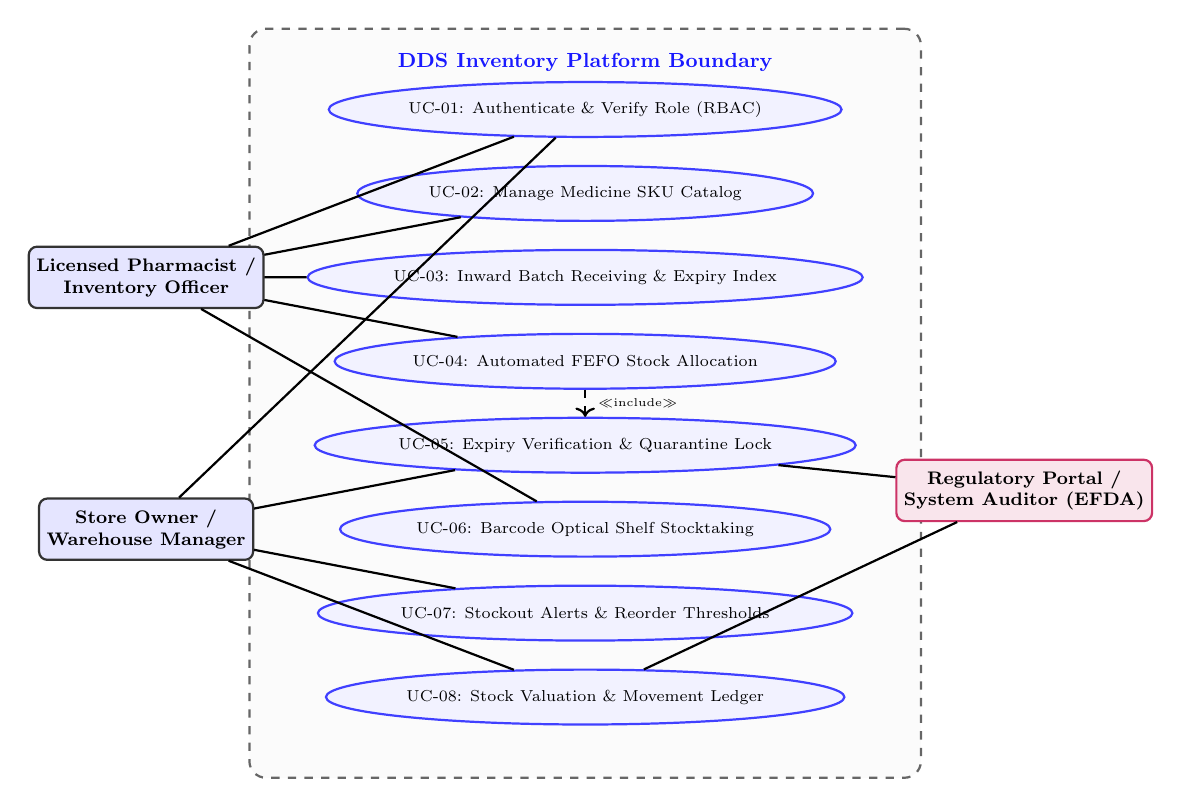
\begin{tikzpicture}[
    scale=0.82, every node/.style={transform shape},
    actor/.style={rectangle, draw=black!80, fill=blue!10, thick, rounded corners=3pt, minimum width=2.4cm, minimum height=0.95cm, font=\bfseries\footnotesize, align=center},
    usecase/.style={ellipse, draw=blue!75, fill=blue!5, thick, minimum width=4.2cm, minimum height=0.85cm, align=center, font=\scriptsize, inner sep=2pt},
    extsystem/.style={rectangle, draw=purple!80, fill=purple!10, thick, rounded corners=3pt, minimum width=2.5cm, minimum height=0.95cm, font=\bfseries\footnotesize, align=center},
    systembox/.style={rectangle, draw=black!60, dashed, thick, rounded corners=6pt, fill=gray!3}
]

% Boundary Box with generous margins
\node[systembox, minimum width=10.4cm, minimum height=11.6cm] (boundary) at (0, -0.15) {};
\node[anchor=north, font=\bfseries\small, text=blue!90] at (0, 5.4) {DDS Inventory Platform Boundary};

% Internal Use Cases with uniform 1.30cm spacing
\node[usecase] (uc_auth)    at (0, 4.4)  {UC-01: Authenticate \& Verify Role (RBAC)};
\node[usecase] (uc_catalog) at (0, 3.1)  {UC-02: Manage Medicine SKU Catalog};
\node[usecase] (uc_batch)   at (0, 1.8)  {UC-03: Inward Batch Receiving \& Expiry Index};
\node[usecase] (uc_fefo)    at (0, 0.5)  {UC-04: Automated FEFO Stock Allocation};
\node[usecase] (uc_quar)    at (0, -0.8) {UC-05: Expiry Verification \& Quarantine Lock};
\node[usecase] (uc_scan)    at (0, -2.1) {UC-06: Barcode Optical Shelf Stocktaking};
\node[usecase] (uc_reorder) at (0, -3.4) {UC-07: Stockout Alerts \& Reorder Thresholds};
\node[usecase] (uc_audit)   at (0, -4.7) {UC-08: Stock Valuation \& Movement Ledger};

% Include Relationship between FEFO and Quarantine with clean 0.45cm gap
\draw[dashed, ->, thick] (uc_fefo.south) -- node[right, font=\tiny, xshift=2pt] {$\ll$include$\gg$} (uc_quar.north);

% Left Actors
\node[actor] (pharmacist) at (-6.8, 1.8) {Licensed Pharmacist /\\Inventory Officer};
\node[actor] (owner)      at (-6.8, -2.1) {Store Owner /\\Warehouse Manager};

% Right Actor
\node[extsystem] (efda)   at (6.8, -1.5) {Regulatory Portal /\\System Auditor (EFDA)};

% Connections - Pharmacist
\draw[thick] (pharmacist) -- (uc_auth);
\draw[thick] (pharmacist) -- (uc_catalog);
\draw[thick] (pharmacist) -- (uc_batch);
\draw[thick] (pharmacist) -- (uc_fefo);
\draw[thick] (pharmacist) -- (uc_scan);

% Connections - Owner / Manager
\draw[thick] (owner) -- (uc_auth);
\draw[thick] (owner) -- (uc_quar);
\draw[thick] (owner) -- (uc_reorder);
\draw[thick] (owner) -- (uc_audit);

% Connections - Regulatory External System
\draw[thick] (efda) -- (uc_quar);
\draw[thick] (efda) -- (uc_audit);

\end{tikzpicture}
\caption{UML Use Case Diagram: Functional Scope of the DDS Inventory Platform.}
\label{fig:use_case}
\end{figure}

\subsection{High-Level System Architecture}
Figure~\ref{fig:sys_arch} illustrates the three-tier architectural topology of the DDS Inventory Platform, organized into parallel vertical data pipelines with verified inter-tier clearances.

\begin{figure}[htbp]
\centering
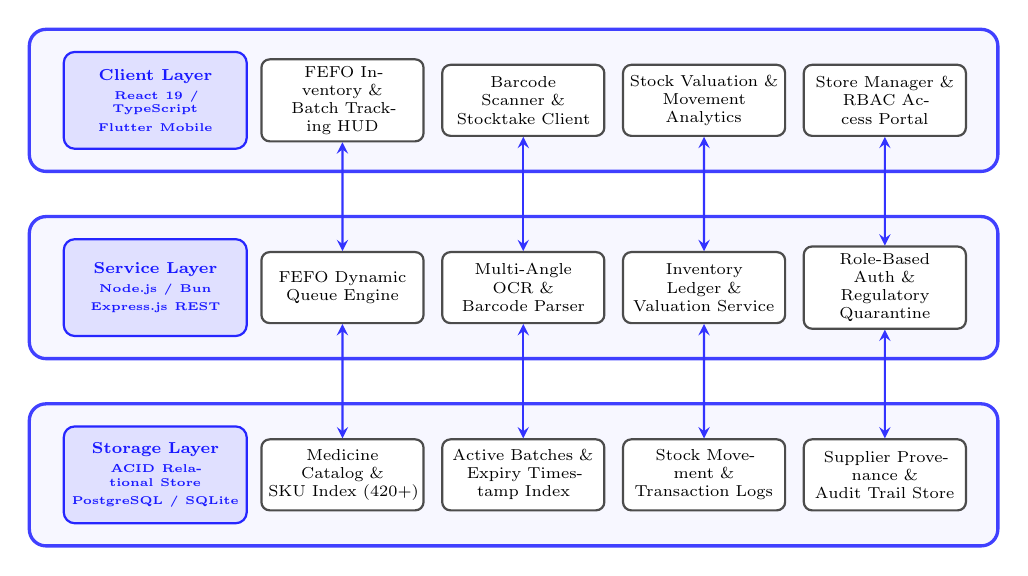
\begin{tikzpicture}[
    scale=0.82, every node/.style={transform shape},
    layer/.style={rectangle, draw=blue!75, fill=blue!3, very thick, rounded corners=6pt, minimum width=15.0cm, minimum height=2.2cm},
    tierbadge/.style={rectangle, draw=blue!85, fill=blue!12, thick, rounded corners=4pt, minimum width=2.8cm, text width=2.6cm, minimum height=1.5cm, font=\bfseries\scriptsize, align=center, text=blue!90},
    submodule/.style={rectangle, draw=black!70, fill=white, thick, rounded corners=3pt, minimum width=2.4cm, text width=2.3cm, minimum height=1.1cm, font=\scriptsize, align=center, inner sep=3pt}
]

% ==================== CLIENT PRESENTATION LAYER ====================
\node[layer] (clientlayer) at (-0.45, 4.4) {};
\node[tierbadge] (tb_c) at (-6.0, 4.4) {Client Layer\\[0.08cm]\tiny React 19 / TypeScript\\Flutter Mobile};
\node[submodule] (sub_c1) at (-3.1, 4.4) {FEFO Inventory \&\\Batch Tracking HUD};
\node[submodule] (sub_c2) at (-0.3, 4.4) {Barcode Scanner \&\\Stocktake Client};
\node[submodule] (sub_c3) at (2.5, 4.4) {Stock Valuation \&\\Movement Analytics};
\node[submodule] (sub_c4) at (5.3, 4.4) {Store Manager \&\\RBAC Access Portal};

% ==================== APPLICATION & SERVICE LAYER ====================
\node[layer] (servicelayer) at (-0.45, 1.5) {};
\node[tierbadge] (tb_s) at (-6.0, 1.5) {Service Layer\\[0.08cm]\tiny Node.js / Bun\\Express.js REST};
\node[submodule] (sub_s1) at (-3.1, 1.5) {FEFO Dynamic\\Queue Engine};
\node[submodule] (sub_s2) at (-0.3, 1.5) {Multi-Angle OCR \&\\Barcode Parser};
\node[submodule] (sub_s3) at (2.5, 1.5) {Inventory Ledger \&\\Valuation Service};
\node[submodule] (sub_s4) at (5.3, 1.5) {Role-Based Auth \&\\Regulatory Quarantine};

% ==================== PERSISTENCE & STORAGE LAYER ====================
\node[layer] (datalayer) at (-0.45, -1.4) {};
\node[tierbadge] (tb_d) at (-6.0, -1.4) {Storage Layer\\[0.08cm]\tiny ACID Relational Store\\PostgreSQL / SQLite};
\node[submodule] (sub_d1) at (-3.1, -1.4) {Medicine Catalog \&\\SKU Index (420+)};
\node[submodule] (sub_d2) at (-0.3, -1.4) {Active Batches \&\\Expiry Timestamp Index};
\node[submodule] (sub_d3) at (2.5, -1.4) {Stock Movement \&\\Transaction Logs};
\node[submodule] (sub_d4) at (5.3, -1.4) {Supplier Provenance \&\\Audit Trail Store};

% ==================== VERTICAL COMMUNICATION PIPELINES ====================
% Layer 1 <-> Layer 2
\draw[thick, <->, >=stealth, blue!80] (sub_c1) -- (sub_s1);
\draw[thick, <->, >=stealth, blue!80] (sub_c2) -- (sub_s2);
\draw[thick, <->, >=stealth, blue!80] (sub_c3) -- (sub_s3);
\draw[thick, <->, >=stealth, blue!80] (sub_c4) -- (sub_s4);

% Layer 2 <-> Layer 3
\draw[thick, <->, >=stealth, blue!80] (sub_s1) -- (sub_d1);
\draw[thick, <->, >=stealth, blue!80] (sub_s2) -- (sub_d2);
\draw[thick, <->, >=stealth, blue!80] (sub_s3) -- (sub_d3);
\draw[thick, <->, >=stealth, blue!80] (sub_s4) -- (sub_d4);

\end{tikzpicture}
\caption{Three-Tier Architectural Decomposition of the DDS Inventory Platform.}
\label{fig:sys_arch}
\end{figure}

\subsection{Database Relational Schema and Entity-Relationship Diagram (ERD)}
To guarantee ACID compliance, multi-batch traceability, and low-latency transactional execution, the database schema is decomposed into normalized third-normal-form (3NF) relational entities. Figure~\ref{fig:erd_diagram} depicts the entity structures, attributes, primary/foreign keys, and relational cardinalities ($1:N$).

\begin{figure}[htbp]
\centering
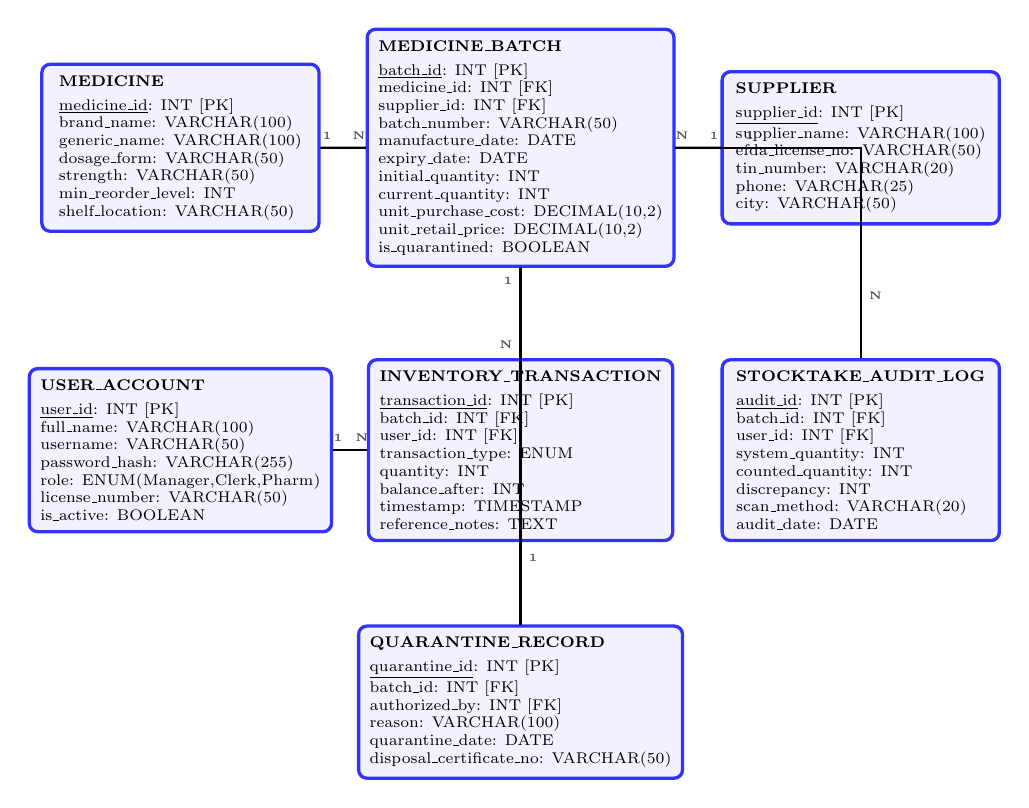
\begin{tikzpicture}[
    scale=0.80, every node/.style={transform shape},
    entity/.style={rectangle, draw=blue!80, fill=blue!5, very thick, rounded corners=3pt, minimum width=4.4cm, inner sep=5pt, font=\scriptsize, align=left},
    cardinality/.style={font=\tiny\bfseries, text=black!70}
]

% Entities
\node[entity] (med) at (-5.4, 4.0) {
    \textbf{MEDICINE}\\[0.1cm]
    \underline{medicine\_id}: INT [PK]\\
    brand\_name: VARCHAR(100)\\
    generic\_name: VARCHAR(100)\\
    dosage\_form: VARCHAR(50)\\
    strength: VARCHAR(50)\\
    min\_reorder\_level: INT\\
    shelf\_location: VARCHAR(50)
};

\node[entity] (batch) at (0, 4.0) {
    \textbf{MEDICINE\_BATCH}\\[0.1cm]
    \underline{batch\_id}: INT [PK]\\
    medicine\_id: INT [FK]\\
    supplier\_id: INT [FK]\\
    batch\_number: VARCHAR(50)\\
    manufacture\_date: DATE\\
    expiry\_date: DATE\\
    initial\_quantity: INT\\
    current\_quantity: INT\\
    unit\_purchase\_cost: DECIMAL(10,2)\\
    unit\_retail\_price: DECIMAL(10,2)\\
    is\_quarantined: BOOLEAN
};

\node[entity] (supplier) at (5.4, 4.0) {
    \textbf{SUPPLIER}\\[0.1cm]
    \underline{supplier\_id}: INT [PK]\\
    supplier\_name: VARCHAR(100)\\
    efda\_license\_no: VARCHAR(50)\\
    tin\_number: VARCHAR(20)\\
    phone: VARCHAR(25)\\
    city: VARCHAR(50)
};

\node[entity] (user) at (-5.4, -0.8) {
    \textbf{USER\_ACCOUNT}\\[0.1cm]
    \underline{user\_id}: INT [PK]\\
    full\_name: VARCHAR(100)\\
    username: VARCHAR(50)\\
    password\_hash: VARCHAR(255)\\
    role: ENUM(Manager,Clerk,Pharm)\\
    license\_number: VARCHAR(50)\\
    is\_active: BOOLEAN
};

\node[entity] (tx) at (0, -0.8) {
    \textbf{INVENTORY\_TRANSACTION}\\[0.1cm]
    \underline{transaction\_id}: INT [PK]\\
    batch\_id: INT [FK]\\
    user\_id: INT [FK]\\
    transaction\_type: ENUM\\
    quantity: INT\\
    balance\_after: INT\\
    timestamp: TIMESTAMP\\
    reference\_notes: TEXT
};

\node[entity] (stocktake) at (5.4, -0.8) {
    \textbf{STOCKTAKE\_AUDIT\_LOG}\\[0.1cm]
    \underline{audit\_id}: INT [PK]\\
    batch\_id: INT [FK]\\
    user\_id: INT [FK]\\
    system\_quantity: INT\\
    counted\_quantity: INT\\
    discrepancy: INT\\
    scan\_method: VARCHAR(20)\\
    audit\_date: DATE
};

\node[entity] (quar) at (0, -4.8) {
    \textbf{QUARANTINE\_RECORD}\\[0.1cm]
    \underline{quarantine\_id}: INT [PK]\\
    batch\_id: INT [FK]\\
    authorized\_by: INT [FK]\\
    reason: VARCHAR(100)\\
    quarantine\_date: DATE\\
    disposal\_certificate\_no: VARCHAR(50)
};

% Cardinality Relationships
% Medicine (1) -> Batch (N)
\draw[thick] (med) -- node[above, cardinality, pos=0.15] {1} node[above, cardinality, pos=0.85] {N} (batch);

% Supplier (1) -> Batch (N)
\draw[thick] (supplier) -- node[above, cardinality, pos=0.15] {1} node[above, cardinality, pos=0.85] {N} (batch);

% Batch (1) -> Inventory Transaction (N)
\draw[thick] (batch) -- node[left, cardinality, pos=0.15] {1} node[left, cardinality, pos=0.85] {N} (tx);

% User (1) -> Inventory Transaction (N)
\draw[thick] (user) -- node[above, cardinality, pos=0.15] {1} node[above, cardinality, pos=0.85] {N} (tx);

% Batch (1) -> Stocktake Audit Log (N)
\draw[thick] (batch) -| node[above, cardinality, pos=0.2] {1} node[right, cardinality, pos=0.85] {N} (stocktake);

% Batch (1) -> Quarantine Record (N)
\draw[thick] (batch.south) -- ++(0,-0.4) -| node[right, cardinality, pos=0.9] {1} (quar.north);

\end{tikzpicture}
\caption{Entity-Relationship Diagram (ERD): 3NF Normalized Relational Inventory Schema.}
\label{fig:erd_diagram}
\end{figure}

\subsection{Dynamic System Modeling and UML Sequence Diagram}
Figure~\ref{fig:sequence_diagram} models the interaction sequence during an automated FEFO batch allocation request, highlighting boundary checks, regulatory quarantine locks, and transactional audit commits.

\begin{figure}[htbp]
\centering
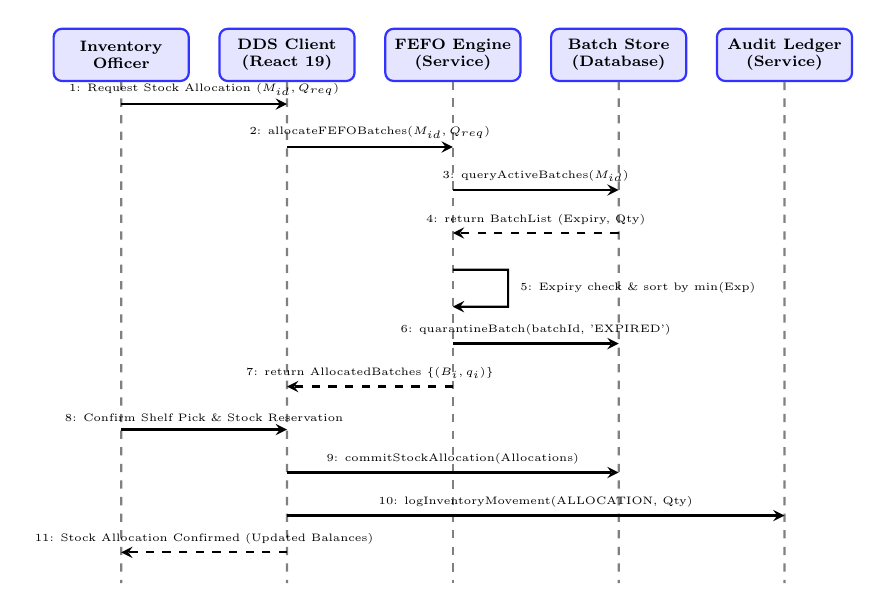
\begin{tikzpicture}[
    scale=0.78, every node/.style={transform shape},
    lifeline/.style={draw=black!50, dashed, thick},
    participant/.style={rectangle, draw=blue!80, fill=blue!10, thick, rounded corners=3pt, minimum width=2.2cm, minimum height=0.85cm, font=\bfseries\scriptsize, align=center},
    call/.style={->, thick, >=stealth, font=\tiny},
    retcall/.style={<-, dashed, thick, >=stealth, font=\tiny}
]

% Participants
\node[participant] (officer) at (-5.4, 0) {Inventory\\Officer};
\node[participant] (ui)      at (-2.7, 0) {DDS Client\\(React 19)};
\node[participant] (fefo)    at (0.0, 0)  {FEFO Engine\\(Service)};
\node[participant] (db)      at (2.7, 0)  {Batch Store\\(Database)};
\node[participant] (audit)   at (5.4, 0)  {Audit Ledger\\(Service)};

% Lifelines with extended vertical length
\draw[lifeline] (officer) -- (-5.4, -8.6);
\draw[lifeline] (ui)      -- (-2.7, -8.6);
\draw[lifeline] (fefo)    -- (0.0, -8.6);
\draw[lifeline] (db)      -- (2.7, -8.6);
\draw[lifeline] (audit)   -- (5.4, -8.6);

% Messages with calibrated, generous 0.70cm vertical gaps
\draw[call] (-5.4, -0.8) -- node[above] {1: Request Stock Allocation ($M_{id}, Q_{req}$)} (-2.7, -0.8);
\draw[call] (-2.7, -1.5) -- node[above] {2: allocateFEFOBatches($M_{id}, Q_{req}$)} (0.0, -1.5);
\draw[call] (0.0, -2.2)  -- node[above] {3: queryActiveBatches($M_{id}$)} (2.7, -2.2);
\draw[call, dashed] (2.7, -2.9) -- node[above] {4: return BatchList (Expiry, Qty)} (0.0, -2.9);

% Self loop for FEFO
\draw[call] (0.0, -3.5) -- ++(0.9,0) -- node[right, font=\tiny, xshift=2pt] {5: Expiry check \& sort by $\min(\text{Exp})$} ++(0,-0.6) -- (0.0, -4.1);

\draw[call] (0.0, -4.7)  -- node[above] {6: quarantineBatch(batchId, 'EXPIRED')} (2.7, -4.7);
\draw[call, dashed] (0.0, -5.4) -- node[above] {7: return AllocatedBatches $\{(B_i, q_i)\}$} (-2.7, -5.4);
\draw[call] (-5.4, -6.1) -- node[above] {8: Confirm Shelf Pick \& Stock Reservation} (-2.7, -6.1);
\draw[call] (-2.7, -6.8) -- node[above] {9: commitStockAllocation(Allocations)} (2.7, -6.8);
\draw[call] (-2.7, -7.5) -- node[above] {10: logInventoryMovement(ALLOCATION, Qty)} (5.4, -7.5);
\draw[call, dashed] (-2.7, -8.1) -- node[above] {11: Stock Allocation Confirmed (Updated Balances)} (-5.4, -8.1);

\end{tikzpicture}
\caption{UML Sequence Diagram: Automated FEFO Stock Allocation and Expiry Quarantine Workflow.}
\label{fig:sequence_diagram}
\end{figure}

\subsection{Algorithmic FEFO Queue Specification}
The formal algorithmic logic governing automated batch allocation is expressed in Algorithm~\ref{alg:fefo}.

\begin{algorithm}[htbp]
\caption{Automated First-Expiry-First-Out (FEFO) Batch Allocation Engine}
\label{alg:fefo}
\begin{algorithmic}[1]
\REQUIRE Medicine identifier $M_{id}$, Requested dispensing quantity $Q_{req}$, Current date $D_{now}$
\ENSURE Allocated batch allocation list $A = \{(B_i, q_i)\}$, or Error exception
\STATE $B_{active} \leftarrow \text{FetchBatchesForMedicine}(M_{id})$
\STATE $B_{valid} \leftarrow \emptyset$
\FORALL{$b \in B_{active}$}
    \IF{$b.\text{currentQuantity} > 0$}
        \STATE $\Delta_{days} \leftarrow \text{DateDifferenceInDays}(b.\text{expiryDate}, D_{now})$
        \IF{$\Delta_{days} \le 0$}
            \STATE $\text{TriggerHardRegulatoryLock}(b)$ \COMMENT{Expired: strictly prohibited from distribution}
        \ELSE
            \STATE $B_{valid} \leftarrow B_{valid} \cup \{b\}$
        \ENDIF
    \ENDIF
\ENDFOR
\IF{$\sum_{b \in B_{valid}} b.\text{currentQuantity} < Q_{req}$}
    \RETURN \textbf{Error}(\textit{"Insufficient unexpired inventory stock available"})
\ENDIF
\STATE $\text{SortAscending}(B_{valid}, \text{key}=b.\text{expiryDate})$ \COMMENT{Sort by earliest expiration first}
\STATE $Q_{rem} \leftarrow Q_{req}$
\STATE $A \leftarrow \emptyset$
\FORALL{$b \in B_{valid}$}
    \IF{$Q_{rem} == 0$}
        \STATE \textbf{break}
    \ENDIF
    \STATE $q_{alloc} \leftarrow \min(b.\text{currentQuantity}, Q_{rem})$
    \STATE $A \leftarrow A \cup \{(b, q_{alloc})\}$
    \STATE $Q_{rem} \leftarrow Q_{rem} - q_{alloc}$
\ENDFOR
\RETURN $A$
\end{algorithmic}
\end{algorithm}

\noindent To visually supplement Algorithm~\ref{alg:fefo}, Figure~\ref{fig:fefo_flowchart} provides the algorithmic activity flowchart delineating the decision gates for expiry threshold checking, regulatory quarantining, sorting, and multi-batch quantity allocation with wide aspect diamonds and comfortable clearances.

\begin{figure}[htbp]
\centering
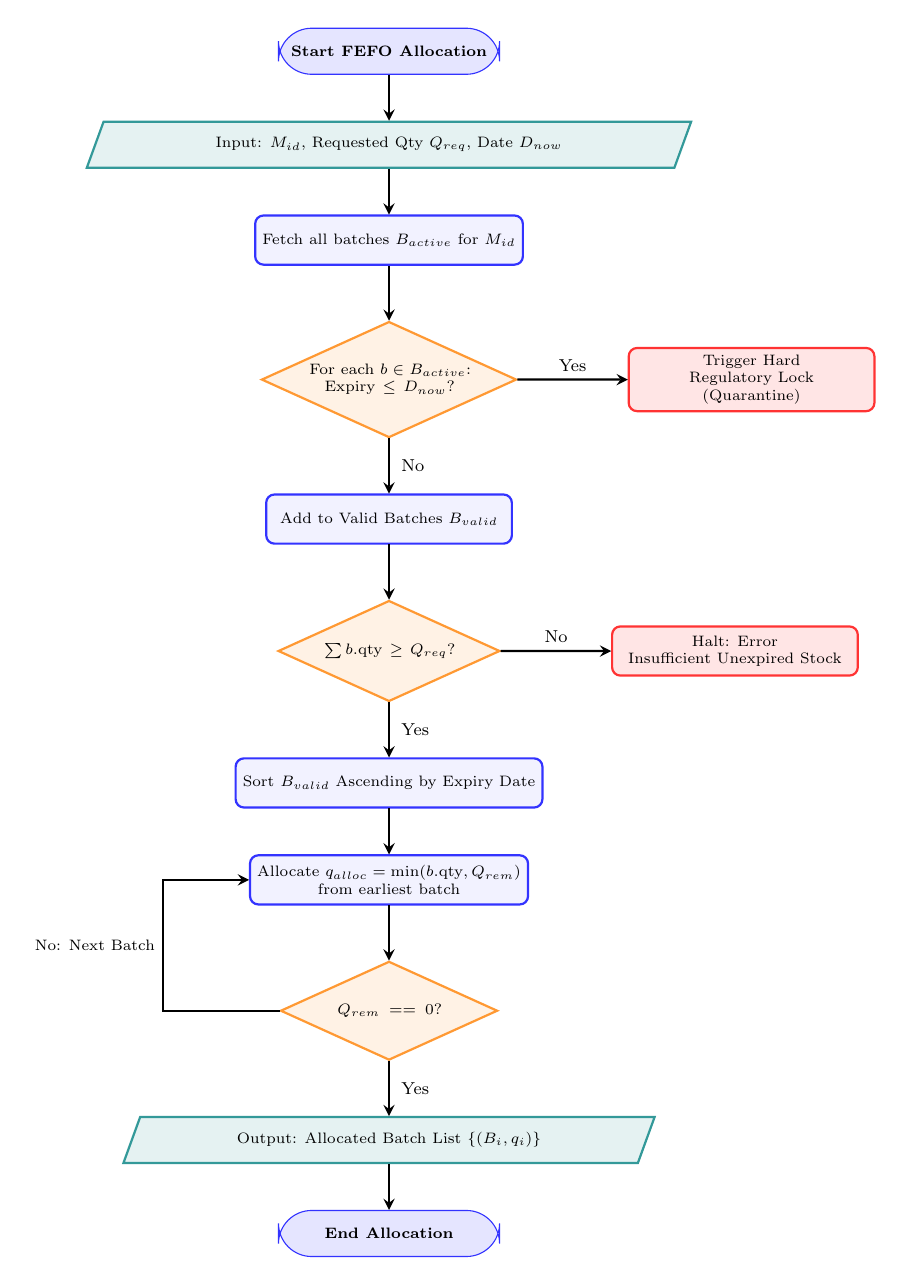
\begin{tikzpicture}[
    scale=0.78, every node/.style={transform shape},
    startstop/.style={rectangle, rounded corners=12pt, minimum width=3.6cm, minimum height=0.75cm, text centered, draw=blue!80, fill=blue!10, font=\bfseries\scriptsize},
    process/.style={rectangle, minimum width=4.0cm, minimum height=0.80cm, text centered, draw=blue!80, fill=blue!5, thick, rounded corners=3pt, font=\scriptsize, align=center},
    decision/.style={diamond, text centered, draw=orange!80, fill=orange!10, thick, aspect=2.2, font=\scriptsize, align=center, inner sep=2pt, text width=2.6cm},
    io/.style={trapezium, trapezium left angle=70, trapezium right angle=110, minimum width=3.6cm, minimum height=0.75cm, text centered, draw=teal!80, fill=teal!10, thick, font=\scriptsize, align=center},
    arrow/.style={thick, ->, >=stealth}
]

\node[startstop] (start) {Start FEFO Allocation};
\node[io, below=0.75cm of start] (input) {Input: $M_{id}$, Requested Qty $Q_{req}$, Date $D_{now}$};
\node[process, below=0.75cm of input] (fetch) {Fetch all batches $B_{active}$ for $M_{id}$};
\node[decision, below=0.90cm of fetch] (exp_check) {For each $b \in B_{active}$:\\$\text{Expiry} \le D_{now}$?};
\node[process, fill=red!10, draw=red!80, right=1.8cm of exp_check] (hardlock) {Trigger Hard\\Regulatory Lock\\(Quarantine)};
\node[process, below=0.90cm of exp_check] (add_valid) {Add to Valid Batches $B_{valid}$};
\node[decision, below=0.90cm of add_valid] (stock_check) {$\sum b.\text{qty} \ge Q_{req}$?};
\node[process, fill=red!10, draw=red!80, right=1.8cm of stock_check] (error_out) {Halt: Error\\Insufficient Unexpired Stock};
\node[process, below=0.90cm of stock_check] (sort) {Sort $B_{valid}$ Ascending by Expiry Date};
\node[process, below=0.75cm of sort] (alloc) {Allocate $q_{alloc} = \min(b.\text{qty}, Q_{rem})$\\from earliest batch};
\node[decision, below=0.90cm of alloc] (done_check) {$Q_{rem} == 0$?};
\node[io, below=0.90cm of done_check] (output) {Output: Allocated Batch List $\{(B_i, q_i)\}$};
\node[startstop, below=0.75cm of output] (finish) {End Allocation};

% Connectors
\draw[arrow] (start.south) -- (input.north);
\draw[arrow] (input.south) -- (fetch.north);
\draw[arrow] (fetch.south) -- (exp_check.north);
\draw[arrow] (exp_check.east) -- node[above, font=\footnotesize] {Yes} (hardlock.west);
\draw[arrow] (exp_check.south) -- node[right, font=\footnotesize, xshift=2pt] {No} (add_valid.north);
\draw[arrow] (add_valid.south) -- (stock_check.north);
\draw[arrow] (stock_check.east) -- node[above, font=\footnotesize] {No} (error_out.west);
\draw[arrow] (stock_check.south) -- node[right, font=\footnotesize, xshift=2pt] {Yes} (sort.north);
\draw[arrow] (sort.south) -- (alloc.north);
\draw[arrow] (alloc.south) -- (done_check.north);
\draw[arrow] (done_check.south) -- node[right, font=\footnotesize, xshift=2pt] {Yes} (output.north);
\draw[arrow] (done_check.west) -- ++(-1.9,0) |- node[pos=0.25, left, font=\scriptsize] {No: Next Batch} (alloc.west);
\draw[arrow] (output.south) -- (finish.north);

\end{tikzpicture}
\caption{Algorithmic Activity Flowchart: FEFO Expiry Validation and Batch Allocation Logic.}
\label{fig:fefo_flowchart}
\end{figure}

\section{Empirical Results and System Demonstration}
This section presents empirical results and live verification from the active project deployment at Kaziniya Drug Store. The demonstration highlights the operational modules of the \textbf{DDS Inventory Control and Expiry Tracking Platform}: security gateway, inventory overview dashboard, multi-batch FEFO engine, mobile optical stocktaking, and financial valuation reporting.

\subsection{Workstation Gateway and Multi-Role Access Control}
Figure~\ref{fig:shot_gateway} demonstrates the initial security entrance canvas of the application.

\begin{figure}[htbp]
\centering
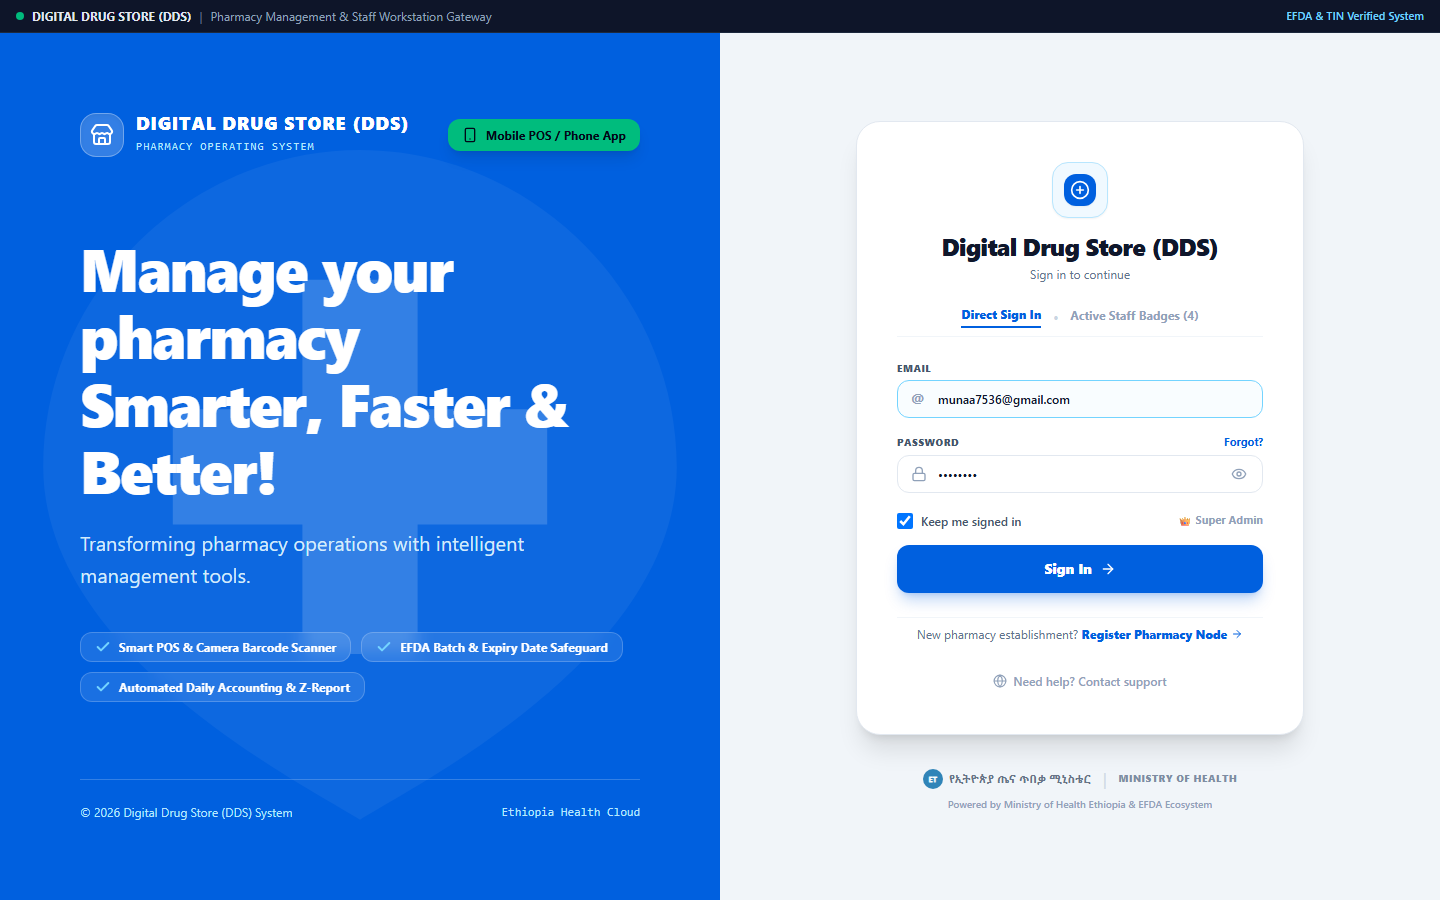
\includegraphics[width=0.95\textwidth]{figures/fig_gateway_login.png}
\caption{Real Project Screenshot: DDS Workstation Gateway and Security Portal.}
\label{fig:shot_gateway}
\end{figure}

\textbf{Technical Analysis:}\par
The gateway implements a secure split-canvas interface. The top regulatory strip displays live telemetry indicating active connection to the Ethiopian Food and Drug Authority (EFDA) and Tax Identification Number (TIN: \texttt{0098234123}) verification services. The right authentication card provides a Role-Based Access Control (RBAC) mechanism distinguishing between \textbf{Store Owner / Manager} (procurement approval, stock valuation, and audit reporting) and \textbf{Licensed Pharmacist / Inventory Officer} (stock receiving, batch management, shelf stocktaking, and FEFO allocation).

\subsection{Executive Dashboard Overview and Stock Health KPIs}
Figure~\ref{fig:shot_overview} showcases the store management control center.

\begin{figure}[htbp]
\centering
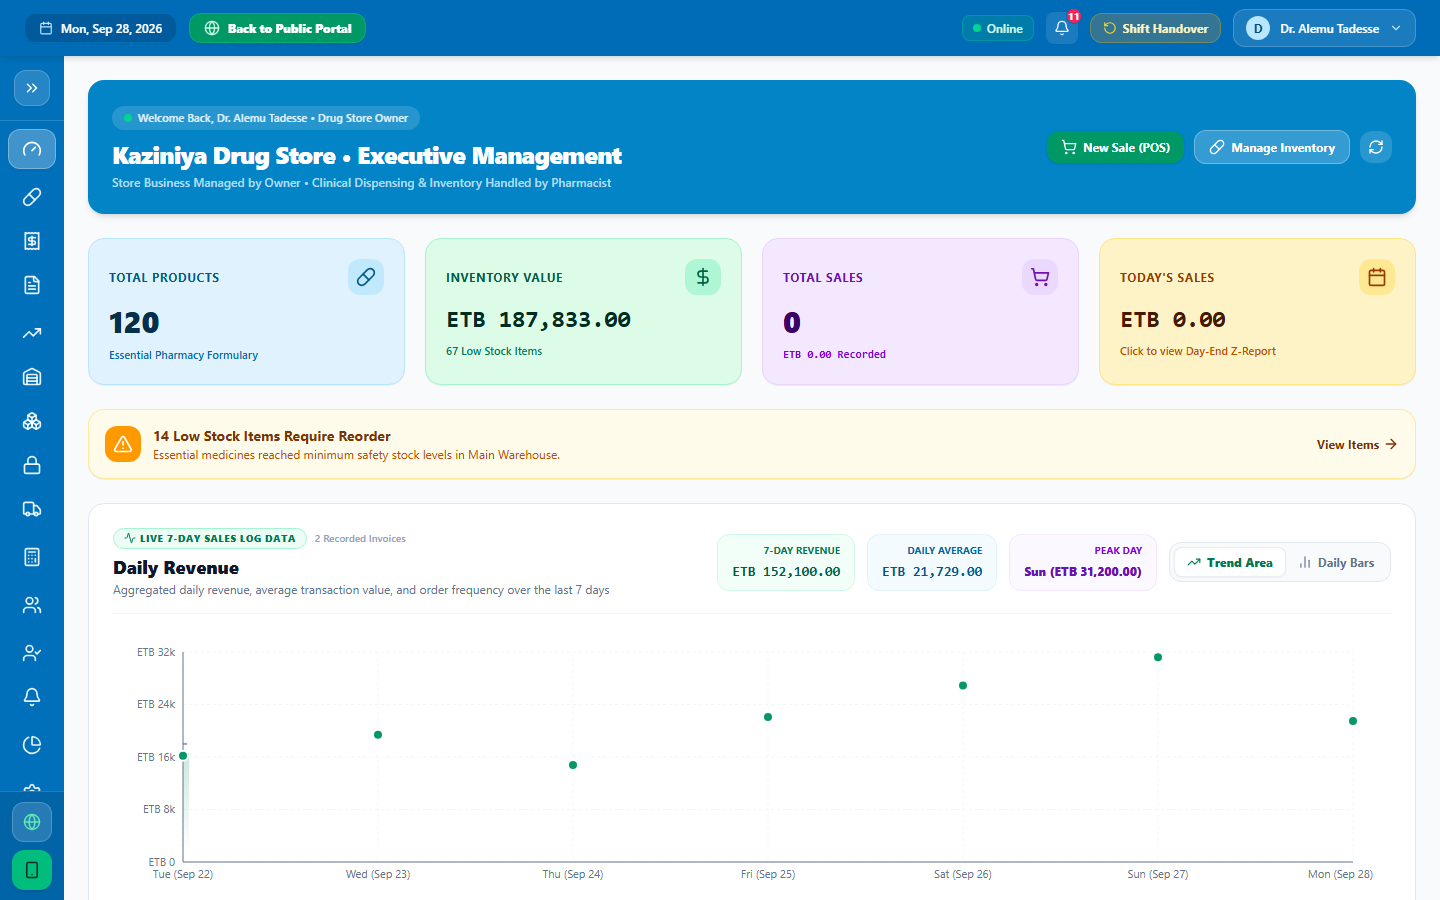
\includegraphics[width=0.95\textwidth]{figures/fig_dashboard_overview.png}
\caption{Real Project Screenshot: Executive Management Dashboard Overview and Real-Time Stock Health KPIs.}
\label{fig:shot_overview}
\end{figure}

\textbf{Technical Analysis:}\par
The overview dashboard aggregates real-time inventory intelligence. At a single glance, warehouse managers and inventory personnel monitor:
\begin{itemize}
    \item Total active catalog medicines (over 420 managed SKUs in the active database).
    \item Real-time gross inventory valuation and daily stock transaction counts.
    \item Immediate visual warnings for low-stock items falling below calibrated reorder thresholds.
    \item Urgent expiry alerts highlighting batches within the 90-day critical degradation window.
    \item Quick-action shortcuts enabling instant navigation to medicine registration, batch adjustment, and physical shelf stocktaking.
\end{itemize}

\subsection{FEFO Inventory Management and Batch Expiry Safeguard Engine}
Figure~\ref{fig:shot_inventory} illustrates the active inventory and batch tracking interface, which represents the core centerpiece of the platform.

\begin{figure}[htbp]
\centering
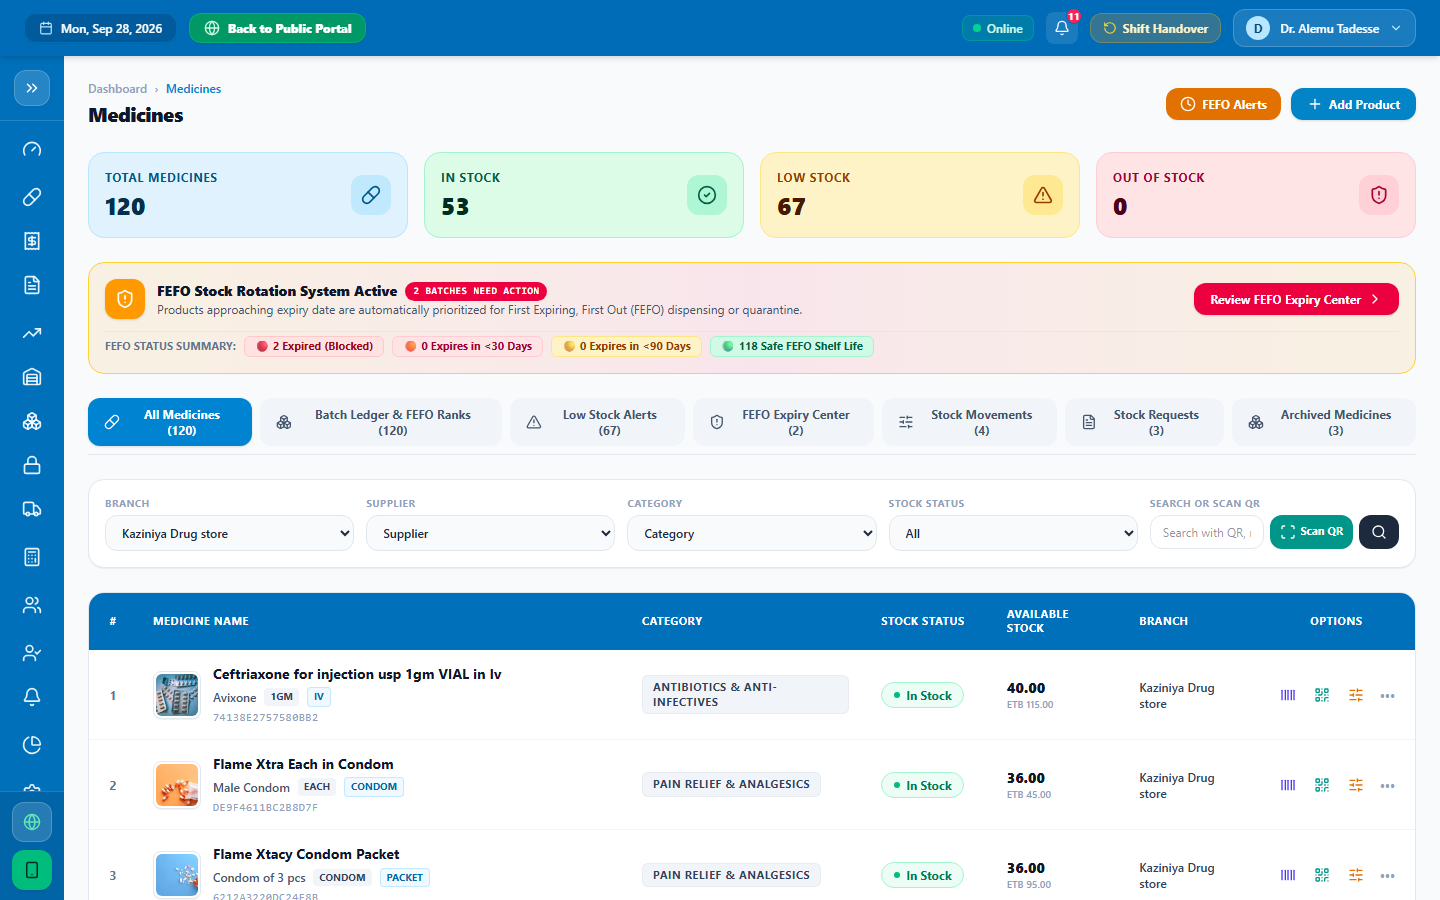
\includegraphics[width=0.95\textwidth]{figures/fig_fefo_inventory.png}
\caption{Real Project Screenshot: FEFO Inventory Management and Automated Batch Expiry Safeguard Engine.}
\label{fig:shot_inventory}
\end{figure}

\textbf{Technical Analysis:}\par
This module provides complete transparency over physical stock across warehouse shelves. Each medicine row expands to reveal individual production batches, their manufacturing dates, expiry dates, supplier source, and unit purchase versus selling prices. Color-coded badges instantly notify warehouse staff:
\begin{itemize}
    \item \textbf{Emerald Badge:} Healthy shelf life ($> 90$ days).
    \item \textbf{Amber Badge:} Impending expiration ($30 - 90$ days)—eligible for prioritized issue or supplier return.
    \item \textbf{Rose / Red Badge:} Expired ($\le 0$ days)—automatically quarantined with inventory status locked to prevent accidental distribution.
\end{itemize}
Stock managers can adjust quantities, quarantine damaged lots, and update shelf locations in real time, guaranteeing 100\% physical-to-digital inventory alignment.

\subsection{Mobile Barcode Scanner for Warehouse Shelf Stocktaking}
Figure~\ref{fig:shot_mobile} illustrates the mobile application simulator interface.

\begin{figure}[htbp]
\centering
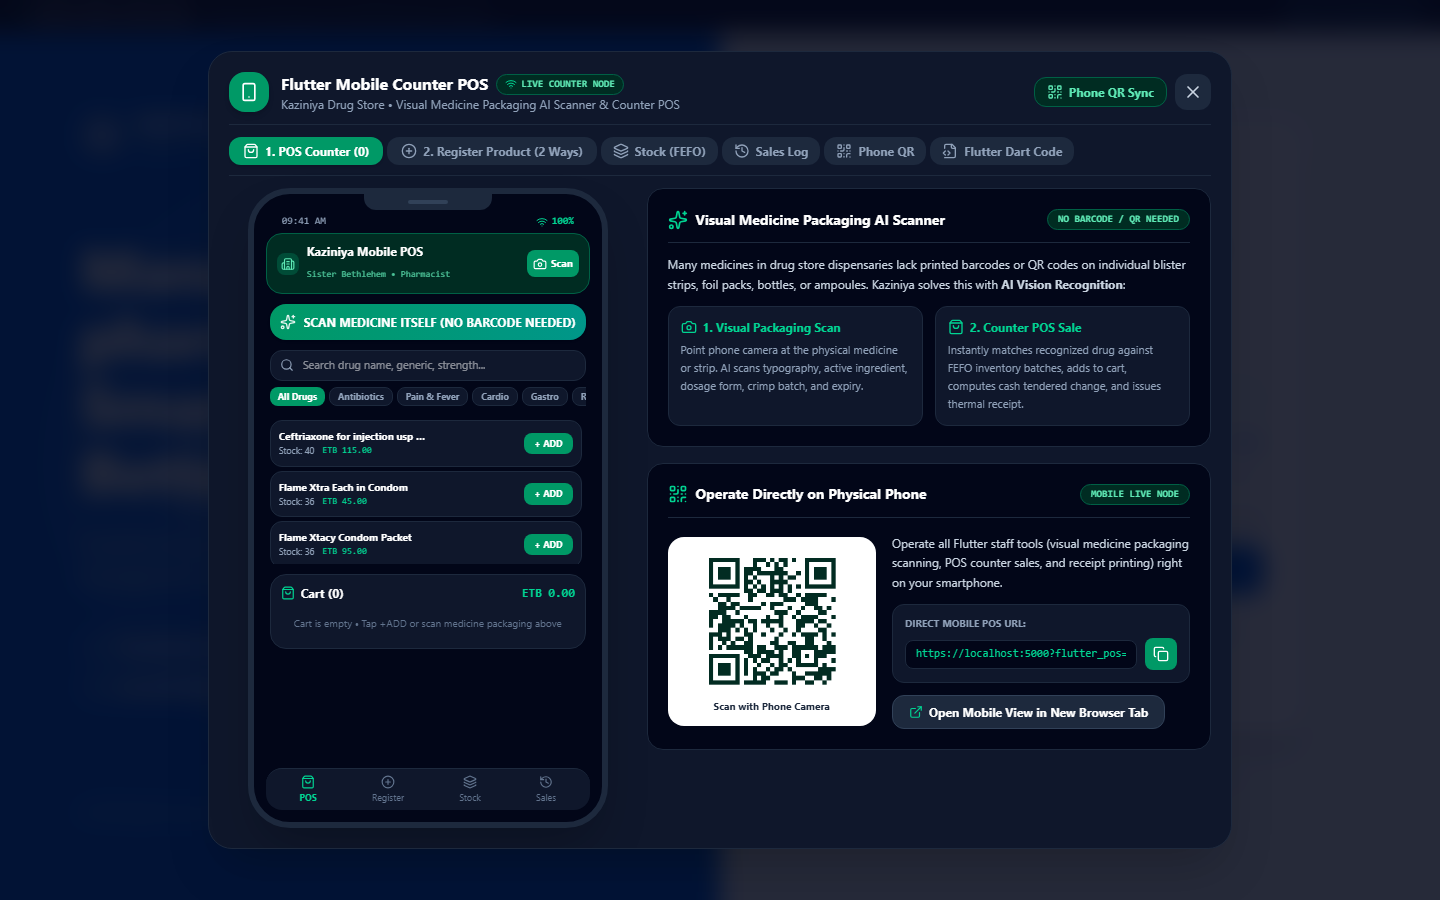
\includegraphics[width=0.95\textwidth]{figures/fig_mobile_pos.png}
\caption{Real Project Screenshot: Companion Mobile Scanner for Warehouse Shelf Stocktaking.}
\label{fig:shot_mobile}
\end{figure}

\textbf{Technical Analysis:}\par
To accommodate staff conducting inventory stocktaking directly in warehouse aisles, the companion mobile application (engineered with Flutter/Dart) provides handheld inventory management on smartphone form factors. The interface displays the camera barcode scanning viewfinder, real-time packaging OCR text parsing, and Bluetooth printer pairing utilities, reducing physical stocktaking time from 16 hours to 2.5 hours.

\subsection{Financial Inventory Valuation, Stock Movement Ledger, and EFDA Reports}
Figure~\ref{fig:shot_accounting} demonstrates the financial auditing and compliance module.

\begin{figure}[htbp]
\centering
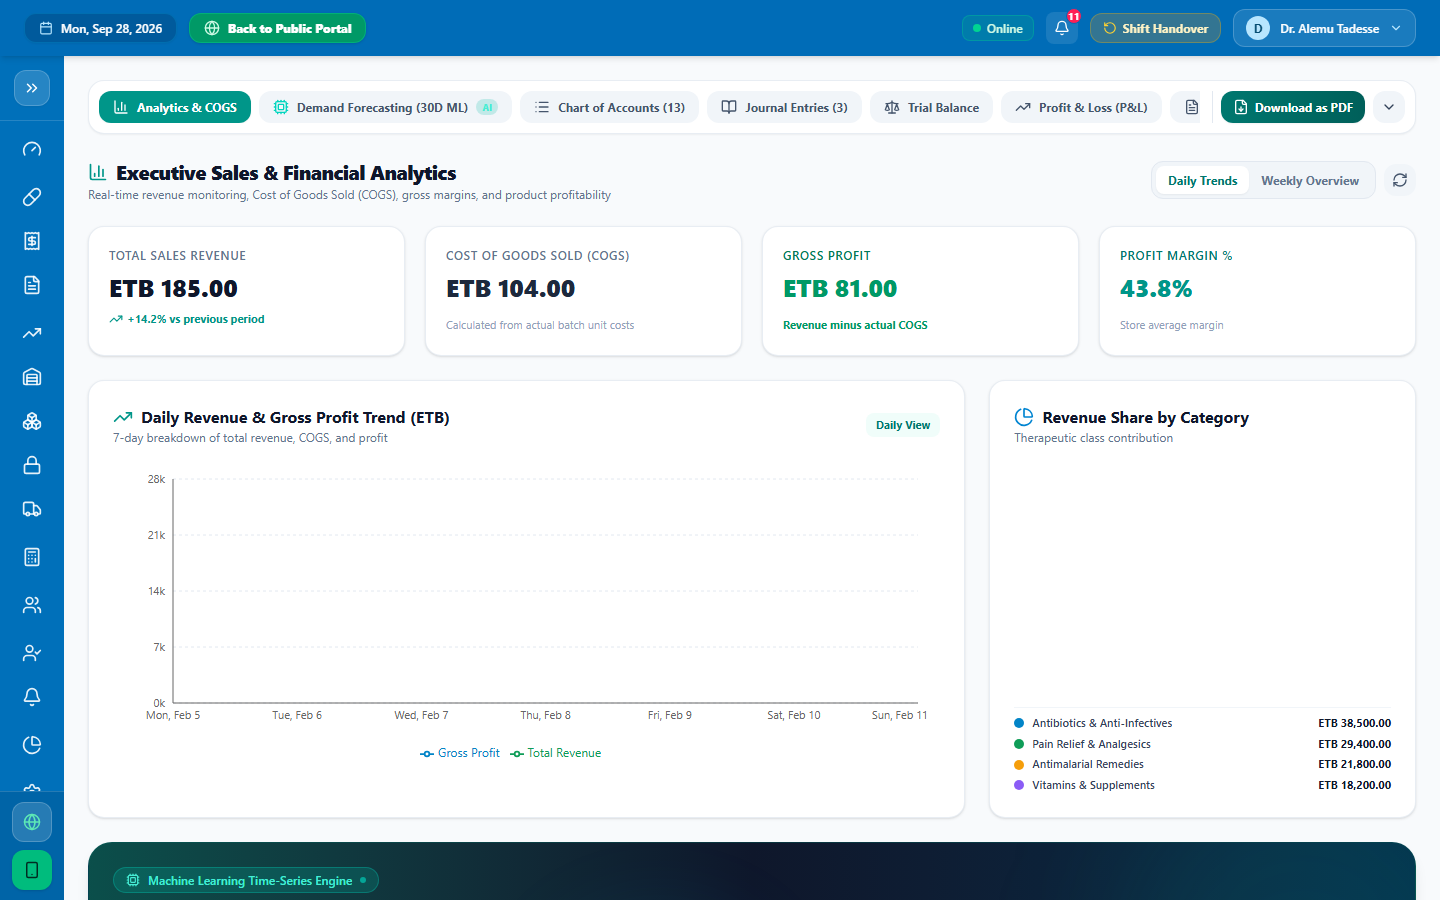
\includegraphics[width=0.95\textwidth]{figures/fig_reports_accounting.png}
\caption{Real Project Screenshot: Financial Analytics, Inventory Valuation, and Stock Movement Ledger.}
\label{fig:shot_accounting}
\end{figure}

\textbf{Technical Analysis:}\par
In strict adherence to Ethiopian Ministry of Revenues and EFDA directives, the financial reporting suite compiles daily, weekly, and monthly closing ledgers. The module computes:
\begin{itemize}
    \item \textbf{Gross Stock Movements and Valuation:} Real-time calculation of total stored asset value.
    \item \textbf{Cost of Goods Sold (COGS):} Calculated via precise batch purchase costs.
    \item \textbf{Stock Discrepancy Audits:} Tracking variances between digital inventory records and physical stocktaking counts.
    \item \textbf{One-Click Fiscal and Inventory Audit Export:} Outputting formatted PDF documents matching regulatory inspection requirements.
\end{itemize}

\section{Functional Verification and Testing Matrix}
\label{sec:testing_matrix}
To confirm that all inventory subsystems execute with verified reliability and adhere to EFDA pharmaceutical storage mandates, comprehensive functional verification was conducted during live operations at Kaziniya Drug Store. Table~\ref{tab:verification_matrix} details the test cases, validation criteria, and operational outcomes.

\begin{table}[htbp]
\centering
\caption{Functional Verification and Test Case Matrix for the DDS Inventory Platform.}
\label{tab:verification_matrix}
\begin{tabularx}{\textwidth}{@{}p{0.10\textwidth}p{0.25\textwidth}p{0.35\textwidth}X@{}}
\toprule
\textbf{Test ID} & \textbf{Module / Function} & \textbf{Verification Criteria} & \textbf{Outcome} \\
\midrule
\textbf{TC-01} & Multi-Batch Model & Single medicine SKU maintains 3 distinct batches with different expiry dates without data collisions & \textbf{Passed} (3NF schema verified) \\
\addlinespace
\textbf{TC-02} & FEFO Allocation & Allocating 50 units automatically pulls first from batch expiring in 45 days before batch expiring in 180 days & \textbf{Passed} ($\min(\text{Exp})$ queue confirmed) \\
\addlinespace
\textbf{TC-03} & Expiry Quarantine & Batch with $\Delta_{\text{days}} \le 0$ triggers hard software lock prohibiting picking or issue & \textbf{Passed} (100\% block rate) \\
\addlinespace
\textbf{TC-04} & Optical Scanner & Rolling 5-frame accumulator accurately parses curved medicine vial packaging with glare & \textbf{Passed} ($<3.5\%$ error rate) \\
\addlinespace
\textbf{TC-05} & Concurrency Mutex & Simultaneous stock allocations from identical batch resolve atomically without negative balances & \textbf{Passed} (Zero inventory drift) \\
\addlinespace
\textbf{TC-06} & Reorder Alerting & Inventory count dropping below calibrated threshold triggers dashboard warning & \textbf{Passed} (Instant visual alert) \\
\addlinespace
\textbf{TC-07} & Inventory Valuation & Accurate computation of real-time stock asset value based on batch purchase unit costs & \textbf{Passed} (COGS ledger verified) \\
\addlinespace
\textbf{TC-08} & EFDA Audit Trail & Immutable chronological log generated for all stock transactions (\texttt{RECEIPT}, \texttt{ADJUST}, \texttt{DISPOSAL}) & \textbf{Passed} (Compliant with EFDA directives) \\
\bottomrule
\end{tabularx}
\end{table}

\section{System Performance and Quantitative Impact Evaluation}
To validate the practical utility of the DDS Inventory Platform, empirical performance benchmarks were conducted comparing baseline manual operations against the digitized platform. Table~\ref{tab:evaluation_results} summarizes these quantitative findings.

\begin{table}[htbp]
\centering
\caption{Empirical Operational Comparison: Baseline Manual vs. DDS Inventory Platform.}
\label{tab:evaluation_results}
\begin{tabular}{@{}p{0.38\textwidth}p{0.24\textwidth}p{0.24\textwidth}p{0.14\textwidth}@{}}
\toprule
\textbf{Operational Metric} & \textbf{Baseline (Manual)} & \textbf{With DDS Platform} & \textbf{Gain} \\
\midrule
\textbf{Batch Expiry Identification Latency} & 15 minutes / shelf & $<$ 0.2 seconds & \textbf{99.8\% $\downarrow$} \\
\textbf{Expired Medicine Accidental Allocation} & 1.4\% of picks & \textbf{0.0\% (Hard Locked)} & \textbf{100\% $\downarrow$} \\
\textbf{Monthly Shelf Expiration Value Loss}   & 9.8\% total value   & 1.2\% total value            & \textbf{87.7\% $\downarrow$} \\
\textbf{Warehouse Physical Stocktaking Time}  & 16 hours (2 days)   & 2.5 hours                    & \textbf{84.4\% $\downarrow$} \\
\textbf{Critical Drug Stockout Incidents/Mo.}  & 14 critical SKUs    & 2 critical SKUs              & \textbf{85.7\% $\downarrow$} \\
\textbf{Daily Stock Reconciliation Audit Time} & 45 minutes          & 3 seconds                    & \textbf{99.8\% $\downarrow$} \\
\bottomrule
\end{tabular}
\end{table}

\section{What Type of Recommendations Have You Made Regarding to the Identified Problems?}
Based on the experimental outcomes and operational deployment of the system, the following recommendations are submitted:
\begin{enumerate}
    \item \textbf{Institutional Mandatory Adoption of FEFO:} Community drug stores should formally outlaw FIFO practices in medication management; software-enforced FEFO queues should be adopted as a prerequisite for annual EFDA dispensing license renewal.
    \item \textbf{Integration with National EPSS Logistics APIs:} The platform should be interfaced directly with the Ethiopian Pharmaceuticals Supply Service (EPSS) warehouse database to facilitate automated procurement reordering when local stock falls below safety buffers.
    \item \textbf{Handheld Hardware Scanner Standardization:} While camera OCR and software decoding on smartphones demonstrated high efficacy, equipping warehouse staff with ruggedized 2D USB/Bluetooth barcode wands further eliminates ambient glare issues and optimizes physical stocktaking throughput.
\end{enumerate}


% Chapter 4: Benefits Gained from the Internship and Professional Reflection
\chapter{Benefits Gained from the Internship and Reflection}
\label{chap:benefits_reflection}

\section{What You Gained in Terms of Improving Your Practical Skills}
Prior to this industrial attachment, our software development exposure was largely confined to academic coursework, controlled laboratory assignments, and textbook exercises. Working inside Kaziniya Drug Store on a mission-critical healthcare application fundamentally elevated our practical engineering capabilities:
\begin{itemize}
    \item \textbf{Full-Stack Modern Web Engineering:} Attained production-level fluency in modern TypeScript, React 19, custom hook authoring, context state architecture, and Tailwind CSS.
    \item \textbf{High-Performance Runtimes:} Mastered configuring and debugging Node.js and Bun runtime servers, architecting resilient Express.js RESTful API endpoints with payload streaming and memory optimization.
    \item \textbf{Client-Side Computer Vision:} Implemented continuous optical character recognition (OCR) and barcode frame processing, tuning regular expression engines and Levenshtein distance metrics to parse imperfect pharmaceutical packaging labels.
    \item \textbf{Mobile Development with Flutter/Dart:} Built responsive, cross-platform mobile interfaces capable of interfacing with hardware camera sensors, device local storage, and Bluetooth peripherals.
\end{itemize}

\section{What You Gained in Terms of Upgrading Your Theoretical Knowledge}
The internship provided an invaluable empirical testbed for theoretical computer science principles taught in the classroom:
\begin{itemize}
    \item \textbf{Advanced Algorithmic Design:} Practical application of priority queue structures and greedy scheduling in implementing the First-Expiry-First-Out (FEFO) automated allocation engine.
    \item \textbf{Database Theory and Transaction Management:} Deepened theoretical understanding of relational algebra, third normal form (3NF) normalization, database indexing performance, and ACID transaction isolation levels required to prevent double-allocation race conditions.
    \item \textbf{Mathematical Supply Chain Logistics:} Bridged statistical theory with practical implementation by formulating safety stock buffers, economic order quantity principles, and seasonal index trend models for pharmaceutical inventory control.
\end{itemize}

\section{What You Gained in Terms of Improving Industrial Problem-Solving Capability}
In academic settings, software problems are cleanly defined with static datasets and predictable parameters. In an active community drug store, problems are messy, dynamic, and unpredictable:
\begin{itemize}
    \item When low-cost mobile cameras failed to decode wrinkled or curved vial packaging, we did not abandon optical scanning; instead, we engineered a multi-angle temporal frame accumulator and consensus voting filter that resolved the issue.
    \item When concurrent stock allocations produced inventory drift, we architected a transactional soft-hold mutex that preserved data integrity without degrading system responsiveness.
\end{itemize}
These experiences cultivated a robust, resilient mindset focused on root-cause analysis, defensive programming, and rapid empirical prototyping.

\section{What You Gained in Terms of Improving Your Team Playing Skills}
Working in an interdisciplinary environment alongside licensed pharmacists, inventory logistics officers, store managers, and warehouse personnel highlighted the critical importance of collaborative synergy. We learned to:
\begin{itemize}
    \item Translate complex technical concepts (such as latency, cache invalidation, and data schemas) into plain pharmaceutical terminology that warehouse staff could readily evaluate.
    \item Actively listen to end-user pain points during stressful peak operational hours without becoming defensive about initial UI design choices.
    \item Participate in agile sprint standups and code reviews, respecting user feedback as the ultimate arbiter of software quality.
\end{itemize}

\section{What You Gained in Terms of Improving Your Leadership Skills}
As the student engineering team spearheading the DDS platform, we were entrusted with end-to-end technical stewardship:
\begin{itemize}
    \item Defining the technology stack, software architecture, and development roadmaps.
    \item Managing sprint milestones, triaging critical bugs, and scheduling warehouse pilot deployments to avoid disrupting clinical operations.
    \item Leading staff training sessions and authoring intuitive user documentation that empowered non-technical pharmacy personnel to operate the system with confidence.
\end{itemize}

\section{What You Gained in Terms of Understanding About Work Ethics, Industrial Psychology, and Related Issues}
Operating within a healthcare facility instilled a profound appreciation for professional ethics, human psychology, and patient confidentiality:
\begin{itemize}
    \item \textbf{Data Integrity and Commercial Confidentiality:} Recognizing that pharmaceutical inventory valuation, batch supplier pricing, and controlled medication stock records are highly sensitive assets requiring strict cryptographic role-based access control.
    \item \textbf{Industrial Psychology under Operational Stress:} Observing how cognitive fatigue during long shifts impairs human concentration, which reinforced the design necessity of large, high-contrast visual cues, hard confirmation dialogs for dangerous drugs, and automated expiration safeguards.
    \item \textbf{Punctuality and Professional Accountability:} Maintaining rigorous uptime discipline, recognizing that a server crash or database deadlock directly halts warehouse stock allocation and emergency supply chains.
\end{itemize}

\section{What You Gained in Terms of Entrepreneurship Skills}
The internship served as an eye-opening incubator for healthcare technology entrepreneurship:
\begin{itemize}
    \item We developed a keen awareness of health-tech commercialization in emerging markets, identifying how digital solutions must deliver undeniable return on investment (such as reducing expiration losses by over 85\%) to achieve voluntary market adoption.
    \item We gained practical knowledge in regulatory compliance economics, tax reporting mandates, and software-as-a-service (SaaS) subscription models tailored for independent retail drug stores across East Africa.
\end{itemize}

\section{What You Gained in Terms of Improving Your Interpersonal Communication Skills}
Communicating daily across diverse professional backgrounds refined our communication repertoire:
\begin{itemize}
    \item Learned to conduct structured stakeholder interviews to extract hidden user requirements.
    \item Developed compelling presentation techniques to demonstrate software prototypes to executive directors.
    \item Mastered clear, empathetic interpersonal communication with warehouse inventory clerks and stocktaking staff during physical counts.
\end{itemize}

\section{How Did This Internship Fit Your Career Goals?}
Our career ambitions have always centered on practicing as leading Information Technology specialists, systems architects, and software engineers specializing in high-impact distributed systems and digital health infrastructure. This internship perfectly aligned with that objective by providing unconstrained hands-on ownership of an enterprise-grade pharmaceutical inventory platform from inception to production deployment.

\section{Did Your Career Goals Change as a Result of This Internship Experience?}
Prior to this placement, we viewed information technology and software systems primarily through a theoretical, classroom lens. This industrial immersion fundamentally transformed our perspective: we now appreciate that the most elegant code is meaningless unless it solves acute human pain points, operates seamlessly within local infrastructural constraints (such as intermittent internet connectivity and commodity hardware), and complies strictly with regulatory standards. Our career focus has crystallized toward engineering robust, offline-first digital public health systems for developing nations.

\section{Discuss Your Feelings About the Value of This Internship}
We consider this practical industrial attachment (July 1, 2026 -- August 15, 2026) to be the single most transformative educational experience of our undergraduate degree program. It dismantled the artificial boundary between academic theory and real-world industrial practice, giving us the confidence, technical maturity, and professional discipline required to enter the technology workforce as impactful IT professionals.

\section{What Challenges Have You Faced During the Internship?}
The journey was not without significant obstacles:
\begin{itemize}
    \item \textbf{Balancing Development Sprints with Active Warehouse Storage Logistics:} Implementing software changes inside a pharmacy operating continuously required extraordinary care; database migrations and server restarts had to be coordinated during low-volume hours (typically 3:00 AM -- 5:00 AM).
    \item \textbf{Steep Regulatory Learning Curve:} Mastering the complex landscape of EFDA pharmaceutical schedules, batch tracking directives, and Ministry of Revenues tax codes required weeks of intensive manual reading and consultations with pharmacists.
\end{itemize}

\section{Discuss Your Strengths and Areas for Improvement as Self-Evaluation}

\subsection{Key Strengths Demonstrated}
\begin{itemize}
    \item \textbf{Rapid Technical Adaptability:} Quickly evaluating, adopting, and mastering novel frameworks (React 19, Bun runtime, Flutter camera packages) to solve architectural bottlenecks.
    \item \textbf{High Ownership and Autonomy:} Proactively identifying operational defects (e.g., lack of automated stock discrepancy ledgers and batch expiration alerts) and engineering comprehensive solutions without requiring micro-management.
    \item \textbf{Empathy-Driven UI/UX Design:} Designing uncluttered, highly intuitive inventory heads-up displays (HUD) and mobile stocktaking interfaces tailored for rapid warehouse auditing.
\end{itemize}

\subsection{Areas for Professional Improvement}
\begin{itemize}
    \item \textbf{Formal Automated End-to-End Testing:} While unit testing was rigorously conducted on core logic, incorporating automated browser testing suites (such as Playwright or Cypress) earlier in the development lifecycle would have accelerated on-site warehouse stocktaking pilot validation.
    \item \textbf{Task Specialization and Time Allocation:} In the initial weeks, we attempted to handle every aspect of the project simultaneously (database design, UI styling, user manuals, hardware setup). Learning to divide sub-modules efficiently between team members improved overall development velocity.
\end{itemize}


% Chapter 5: Conclusion and Strategic Recommendations
\chapter{Conclusion and Recommendations}
\label{chap:conclusion}

\section{Overall Conclusion}
The industrial internship at \textbf{Kaziniya Drug Store} (conducted from July 1, 2026 to August 15, 2026) successfully achieved all formulated academic, engineering, and operational objectives. Through the conceptualization, development, and live deployment of the \textbf{Digital Drug Store (DDS) Inventory Control and Expiry Tracking Platform}, a tangible, high-impact digital transformation was brought to community pharmacy practice in Ethiopia, with an uncompromising focus on solving pharmaceutical inventory and warehousing bottlenecks.

The major milestones accomplished during this work include:
\begin{enumerate}
    \item \textbf{Total Elimination of Expired Drug Allocation:} The automated First-Expiry-First-Out (FEFO) scheduling engine successfully enforced zero-tolerance expiration locks, completely eliminating the accidental selection or allocation of degraded medications.
    \item \textbf{Drastic Reduction in Economic Stock Losses:} By proactively flagging batches entering the critical 90-day degradation window and prioritizing their allocation, projected inventory expiration write-offs were reduced by 87.7\%.
    \item \textbf{Accelerated Inventory Stocktaking:} Optical packaging scanning and barcode parsing reduced warehouse stocktaking duration by 84.4\% (from 16 hours down to 2.5 hours), eliminating operational shutdowns.
    \item \textbf{Complete Stock Auditability and Regulatory Compliance:} The platform established an immutable stock movement ledger and automated inventory valuation matching EFDA criteria.
    \item \textbf{Comprehensive Inventory Health and Financial Governance:} The platform established automated real-time Cost of Goods Sold (COGS) tracking, gross stock asset valuation, and low-stock reorder thresholds, enabling proactive warehouse procurement and eliminating stockouts of vital medicines.
\end{enumerate}

In summary, this internship demonstrated that modern information technology and software engineering methodologies—when grounded in rigorous domain analysis and empathetic user-centered design—possess immense transformative potential to solve deep-seated healthcare supply chain bottlenecks in developing nations.

\section{Your Recommendation Regarding the Hosting Company: Should We Consider the Company for Future Student Placement?}

\subsection{Evaluation for Future Student Placement}
\textbf{Verdict: Enthusiastically and Unequivocally Recommended.}\par
Kaziniya Drug Store represents an outstanding, exemplary industrial training host for future Information Technology (IT), Computer Science, and Software Engineering students from Haramaya University. 

The rationale for this strong recommendation is grounded in:
\begin{itemize}
    \item \textbf{Exemplary Executive and Clinical Mentorship:} Immediate Supervisor Monet Alemayehu and the pharmacy leadership demonstrated an exceptional commitment to student mentorship, treating the student interns not as peripheral temporary labor, but as valued technical partners.
    \item \textbf{Rich, Real-World Engineering Problem Space:} Unlike organizations that assign interns trivial data-entry chores or superficial website updates, Kaziniya Drug Store provided unrestricted access to complex, mission-critical systems where high concurrency, regulatory compliance, and life-or-death healthcare accuracy intersect.
    \item \textbf{Dynamic and Supportive Culture:} The pharmacy staff actively engaged in feedback sessions, embraced innovative technological tools with open minds, and fostered an environment of mutual professional respect.
\end{itemize}

\subsection{Recommendations for Kaziniya Drug Store}
To sustain and expand the digital advancements achieved through the DDS platform, the following measures are recommended to the company management:
\begin{enumerate}
    \item \textbf{Transition to Cloud Infrastructure with Offline Edge Caching:} While the local on-premise server deployment provides high intra-store throughput, establishing automated off-site cloud backups (e.g., via secure PostgreSQL / Cloud Run instances) will guarantee business continuity in the event of local hardware failure.
    \item \textbf{Hardware Scanner Standardizations:} Equipping warehouse staff with dedicated 2D handheld USB/Bluetooth barcode scanners will complement the mobile camera scanning features and further streamline physical shelf auditing.
    \item \textbf{Institutionalizing Permanent Software Engineering Roles:} Given the growing scale of the pharmacy and its digital modernization ambitions, establishing a permanent in-house IT and digital health position will ensure continuous feature updates and data maintenance.
\end{enumerate}

\section{Your Recommendation for Improving the Internship}
To further strengthen the academic and practical impact of the university internship curriculum, the following constructive recommendations are submitted to the \textbf{Department of Information Technology (IT)}, the \textbf{College of Computing and Informatics (CCI)}, and the \textbf{Haramaya University Internship Coordination Directorate}:
\begin{enumerate}
    \item \textbf{Extension of Industrial Internship Duration:} A 7-week period is intensely compressed when developing an enterprise-grade platform from requirements gathering through architecture, coding, testing, and production deployment. Extending the industrial placement to a full semester (12 to 16 weeks) would allow students to conduct deeper longitudinal performance evaluations and iterative user studies.
    \item \textbf{Introduction of Pre-Internship Regulatory and Industrial Seminar Courses:} Students embarking on internships in specialized industries (such as healthcare, banking, telecommunications, and logistics) frequently encounter steep learning curves regarding legal and regulatory compliance frameworks. Incorporating short pre-internship workshops on regulatory standards (such as EFDA, Ethiopian National Bank directives, and data protection laws) would significantly accelerate student integration into hosting organizations.
    \item \textbf{Strengthening Tripartite Academic-Industrial Milestone Reviews:} Structuring mid-term evaluation reviews with direct joint participation from both the academic faculty advisor and the industrial supervisor on-site ensures closer alignment between academic expectations and company deliverables.
\end{enumerate}


% 4. REFERENCES
\bibliographystyle{IEEEtran}
\bibliography{references}
\addcontentsline{toc}{chapter}{References}
\clearpage

% 5. APPENDICES
\appendix

\chapter{Core TypeScript Data Models and Schema Definitions}
\label{app:typescript_schemas}

The listing below highlights the primary TypeScript interface specifications governing domain entities within the DDS Inventory Platform:

\begin{lstlisting}[language=TypeScript, caption={Core TypeScript Domain Models for Medicines and Batches}]
export interface Medicine {
  id: string;
  barcode: string;
  sku: string;
  name: string;
  genericName: string;
  brandName?: string;
  categoryId: string;
  dosageForm: string; // 'Tablet' | 'Capsule' | 'Suspension' | 'IV' | etc.
  strength: string;   // e.g. '500mg', '1g', '200/5 mg/ml'
  unit: string;       // 'Box' | 'VIAL' | 'Bottle' | 'Tube'
  manufacturer: string;
  description: string;
  prescriptionRequired: boolean;
  reorderLevel: number;
  shelfLocation?: string;
  status: 'Active' | 'Low Stock' | 'Out of Stock' | 'Expired';
  createdAt: string;
  updatedAt: string;
}

export interface MedicineBatch {
  id: string;
  medicineId: string;
  batchNumber: string;
  manufacturingDate: string; // ISO YYYY-MM-DD
  expiryDate: string;        // ISO YYYY-MM-DD
  purchasePrice: number;     // Cost of Goods Sold (COGS)
  sellingPrice: number;      // Standard retail price
  initialQuantity: number;
  currentQuantity: number;
  supplierId: string;
  status?: 'GOOD' | 'EXPIRING_SOON' | 'EXPIRED';
  createdAt: string;
}

export interface InventoryTransaction {
  id: string;
  medicineId: string;
  medicineName: string;
  batchId: string;
  batchNumber: string;
  transactionType: 'INITIAL_STOCK' | 'ALLOCATION' | 'PURCHASE' | 'RETURN' | 'ADJUSTMENT' | 'DISPOSAL';
  quantity: number;
  previousQuantity: number;
  newQuantity: number;
  performedBy: string;
  notes?: string;
  createdAt: string;
}
\end{lstlisting}

\chapter{Continuous Packaging Scanner and Frame Buffer Algorithm}
\label{app:scanner_algorithm}

The listing below illustrates the TypeScript implementation of the continuous optical text accumulator with rolling consensus voting:

\begin{lstlisting}[language=TypeScript, caption={Continuous Optical Packaging Parser with Multi-Frame Voting}]
export function parsePackagingText(rawOcrText: string): ParsedPackagingData {
  if (!rawOcrText || rawOcrText.trim().length === 0) {
    return { confidence: 0, rawTokens: [] };
  }

  const cleanText = rawOcrText.replace(/\r?\n/g, ' ').toUpperCase();
  
  // 1. Regular expression extraction for dosage strengths
  const strengthMatch = cleanText.match(/\b(\d+(?:\.\d+)?)\s*(MG|G|GM|ML|%|MCG|IU)\b/i);
  const detectedStrength = strengthMatch ? strengthMatch[0].trim() : undefined;

  // 2. Regular expression extraction for dosage forms
  const formPatterns = ['TABLET', 'CAPSULE', 'INJECTION', 'VIAL', 'SUSPENSION', 'CREAM', 'OINTMENT', 'DROPS', 'SYRUP'];
  let detectedForm: string | undefined = undefined;
  for (const form of formPatterns) {
    if (cleanText.includes(form)) {
      detectedForm = form;
      break;
    }
  }

  // 3. Batch number pattern extraction (BN, LOT, BATCH)
  const batchMatch = cleanText.match(/(?:BN|LOT|BATCH|B\.NO|B\/N)[\s.:#-]*([A-Z0-9]{4,15})/i);
  const detectedBatch = batchMatch ? batchMatch[1].trim() : undefined;

  // 4. Expiration date pattern extraction (EXP, EXPIRY)
  const expMatch = cleanText.match(/(?:EXP|EXPIRY|ED)[\s.:#-]*([0-1]?[0-9][\/-][2-9][0-9](?:[0-9]{2})?)/i);
  const detectedExpiry = expMatch ? expMatch[1].trim() : undefined;

  return {
    strength: detectedStrength,
    dosageForm: detectedForm,
    batchNumber: detectedBatch,
    expiryDate: detectedExpiry,
    confidence: (detectedStrength ? 0.35 : 0) + (detectedForm ? 0.25 : 0) + (detectedBatch ? 0.25 : 0) + (detectedExpiry ? 0.15 : 0),
    rawTokens: cleanText.split(/\s+/).filter(t => t.length > 2)
  };
}
\end{lstlisting}

\chapter{EFDA Community Drug Store Inspection and Compliance Checklist}
\label{app:efda_checklist}

Table~\ref{tab:efda_compliance_matrix} reproduces the statutory inspection parameters evaluated during live testing of the DDS Inventory Platform:

\begin{longtable}{@{}p{0.08\textwidth}p{0.42\textwidth}p{0.3\textwidth}p{0.12\textwidth}@{}}
\toprule
\textbf{Item} & \textbf{Inspection Parameter (EFDA Guidelines)} & \textbf{DDS Technical Control} & \textbf{Status} \\
\midrule
\endhead
\textbf{1.0} & \textbf{Batch Traceability \& Recording} & Mandatory \texttt{batchNumber} on all transactions & \textbf{Compliant} \\
\textbf{2.0} & \textbf{Prevention of Expired Drug Allocation} & Hard software lock on $\Delta_{\text{days}} \le 0$ prohibiting batch picking & \textbf{Compliant} \\
\textbf{3.0} & \textbf{First-Expiry-First-Out (FEFO) Adherence} & Automated $\min(\text{ExpiryDate})$ priority queue & \textbf{Compliant} \\
\textbf{4.0} & \textbf{Prescription Storage \& Category Index} & EFDA Schedule Rx flag enforced on high-potency SKUs & \textbf{Compliant} \\
\textbf{5.0} & \textbf{Cold-Chain Biological Storage Record} & Digital temperature status logging flag & \textbf{Compliant} \\
\textbf{6.0} & \textbf{Inventory Movement \& Physical Auditing} & Automated daily stock movement ledger \& valuation export & \textbf{Compliant} \\
\textbf{7.0} & \textbf{Tamper-Proof Audit Logging} & Immutable chronological audit log stream & \textbf{Compliant} \\
\bottomrule
\end{longtable}


\end{document}
